\documentclass[../../main.tex]{subfiles}
\begin{document}
\section{Validity of the Timoshenko beam model}
This section is a literature study of the article \cite{LVV09}. The goal of \cite{LVV09} to show that the one-dimensional Timoshenko beam theory, is a feasible model to use in practical applications of beams. In the real world, a beam is a complex three-dimensional model. So a three-dimensional model would be a good approximation and better than a one-dimensional model. It is therefore important to validate the accuracy of a simlified theory like the Timoshenko beam theory.\\

In the article, the authors validate the Timoshenko beam theory by comparing it to a more realistic, two-dimensional model. The authors use a cantilever beam as a model. Although a direct comparison to a three-dimensional beam would be preferred, the authors state that this would introduce complexities. The two-dimensional model is an intermediate step.\\

Where \cite{LVV09} differs from most other research into the validity of the Timoshenko beam theory, is that the boundary conditions are also taken into consideration.\\

To compare the two models, the authors compare the natural frequencies of the models. From modal analysis, it is known that a solution of a second order hyperbolic type problem is a linear combination of the eigenvalues and eigenfunctions of the model. Therefore it is sufficient to compare the eigenvalues and eigenfunctions to compare the solutions and comment on the validity of the models.\\

\subsection{The models}
In the article, the authors use a cantilever configuration for the two models. Therefore the models presented here are also cantilever models.\\

Recall the cantilever Timoshenko beam model from section \ref{ssec:1D_Model:ModelProblems}, referred to as Problem T-2 and the cantilever two-dimensional beam model from section \ref{ssec:2D_Model:ModelProblem}, referred to as Problem 2D-1. In \cite{LVV09} it is assumed that the beams have a rectangular cross-section.\\

Figure 6.1 shows the two beams side-by-side.

\begin{figure}[h!]\label{fig:compare:1D+2D}
	\scalebox{.8}{
		\makebox[\textwidth][c]{
			\caption{Side by side comparison of the beams.}
			\centering
			\begin{minipage}[b]{0.8\linewidth}
				\begin{center}
					\begin{tikzpicture}
					\draw[line width = 0.4mm] (0,0) -- (6,0);
					
					\node at (2.7,-0.25) {$\ell = 1$};
					
					\draw[line width = 0.1mm] (0,-1.5) -- (0,1.5);
					\draw[line width = 0.1mm] (0,1.5) -- (-0.2,1.4);
					\draw[line width = 0.1mm] (0,1.3) -- (-0.2,1.2);
					\draw[line width = 0.1mm] (0,1.1) -- (-0.2,1);
					\draw[line width = 0.1mm] (0,0.9) -- (-0.2,0.8);
					\draw[line width = 0.1mm] (0,0.7) -- (-0.2,0.6);
					\draw[line width = 0.1mm] (0,0.5) -- (-0.2,0.4);
					\draw[line width = 0.1mm] (0,0.3) -- (-0.2,0.2);
					\draw[line width = 0.1mm] (0,0.1) -- (-0.2,0);
					
					\draw[line width = 0.1mm] (0,-0.1) -- (-0.2,-0.2);
					\draw[line width = 0.1mm] (0,-0.3) -- (-0.2,-0.4);
					\draw[line width = 0.1mm] (0,-0.5) -- (-0.2,-0.6);
					\draw[line width = 0.1mm] (0,-0.7) -- (-0.2,-0.8);
					\draw[line width = 0.1mm] (0,-0.9) -- (-0.2,-1);
					\draw[line width = 0.1mm] (0,-1.1) -- (-0.2,-1.2);
					\draw[line width = 0.1mm] (0,-1.3) -- (-0.2,-1.4);
					\draw[line width = 0.1mm] (0,-1.5) -- (-0.2,-1.6);
					
					%\node at (3.2,-0.2) {$\ell = 1$};
					\end{tikzpicture}
				\end{center}
				\subcaption{Timoshenko Cantilever Beam}
			\end{minipage}
			\begin{minipage}[b]{0.8\linewidth}
				\begin{center}
					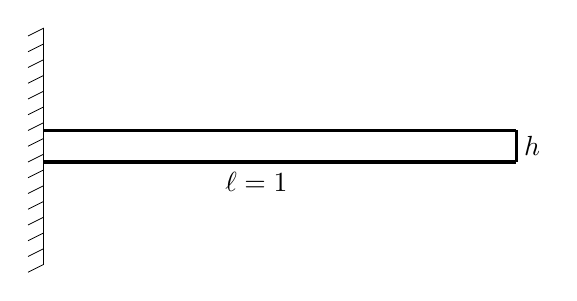
\begin{tikzpicture}
						\draw[line width = 0.4mm] (0,0.2) -- (6,0.2);
						\draw[line width = 0.4mm] (0,-0.2) -- (6,-0.2);
						\draw[line width = 0.4mm] (6,-0.2) -- (6,0.2);
						%\draw[line width = 0.4mm] (0,-0.2) -- (0,0.2);
						
						%\draw[line width = 0.1mm,->] (6,2) -- (7.4,2);
						%\draw[line width = 0.1mm,->] (6,2) -- (6,0.9);
						%\node at (6.7,1.8) {$e_1$};
						%\node at (5.8,1.4) {$e_2$};
						
						\node at (6.2,0) {$h$};
						\node at (2.7,-0.45) {$\ell = 1$};
						
						\draw[line width = 0.1mm] (0,-1.5) -- (0,1.5);
						\draw[line width = 0.1mm] (0,1.5) -- (-0.2,1.4);
						\draw[line width = 0.1mm] (0,1.3) -- (-0.2,1.2);
						\draw[line width = 0.1mm] (0,1.1) -- (-0.2,1);
						\draw[line width = 0.1mm] (0,0.9) -- (-0.2,0.8);
						\draw[line width = 0.1mm] (0,0.7) -- (-0.2,0.6);
						\draw[line width = 0.1mm] (0,0.5) -- (-0.2,0.4);
						\draw[line width = 0.1mm] (0,0.3) -- (-0.2,0.2);
						\draw[line width = 0.1mm] (0,0.1) -- (-0.2,0);
						
						\draw[line width = 0.1mm] (0,-0.1) -- (-0.2,-0.2);
						\draw[line width = 0.1mm] (0,-0.3) -- (-0.2,-0.4);
						\draw[line width = 0.1mm] (0,-0.5) -- (-0.2,-0.6);
						\draw[line width = 0.1mm] (0,-0.7) -- (-0.2,-0.8);
						\draw[line width = 0.1mm] (0,-0.9) -- (-0.2,-1);
						\draw[line width = 0.1mm] (0,-1.1) -- (-0.2,-1.2);
						\draw[line width = 0.1mm] (0,-1.3) -- (-0.2,-1.4);
						\draw[line width = 0.1mm] (0,-1.5) -- (-0.2,-1.6);
						
						%\node at (3.2,-0.3) {$\ell = 1$};
					
					\end{tikzpicture}
				\end{center}
				\subcaption{Two-Dimensional Cantilever Beam}
			\end{minipage}
		}
	}
\end{figure}

In Chapter 1, the following parameters were defined. The parameter $h$ is the height of the two-dimensional beam and for the Timoshenko dimensionless constant $\displaystyle \alpha = \frac{A \ell^2}{I}$ was found.\\

For the Timoshenko beam model with a rectangular cross-section, the area moment of inertial is calculated as
\begin{eqnarray*}
	I = \frac{h^3b}{12}.
\end{eqnarray*}

After substitution, the following relationship between $\alpha$ and $h$ is found
\begin{eqnarray*}
	h = \sqrt{\frac{12}{\alpha}}.
\end{eqnarray*}
Using this relationship, $\alpha$ can be chosen in such a way that the beams have equal lateral dimensions.


\subsection{Accuracy of the numerical eigenvalues}
The calculate the eigenvalues and eigenfunctions of the Timoshenko beam, the authors of \cite{LVV09} use the article \cite{VV06}. This article was discussed in section \ref{sec:Timo:EigenvalueProblem} in this dissertation. It is important to note that the method described in \cite{VV06} allows us to find the eigenvalues of a cantilever Timoshenko beam accurate to a desired level, using numerical methods like interval division.\\

A different approach is needed for the two-dimensional beam. In section \ref{sec:FEM:2D}, the Finite Element Method was used to obtain a numerical formula to solve the eigenvalue problem Problem 2D-1E. In \cite{LVV09} the authors used piecewise bi-cubic basis functions and a grid size large enough to ensure that the eigenvalues are accurate to 3 significant digits.\\

\begin{figure}[H]
	\begin{center}
		\scalebox{1.4}{
			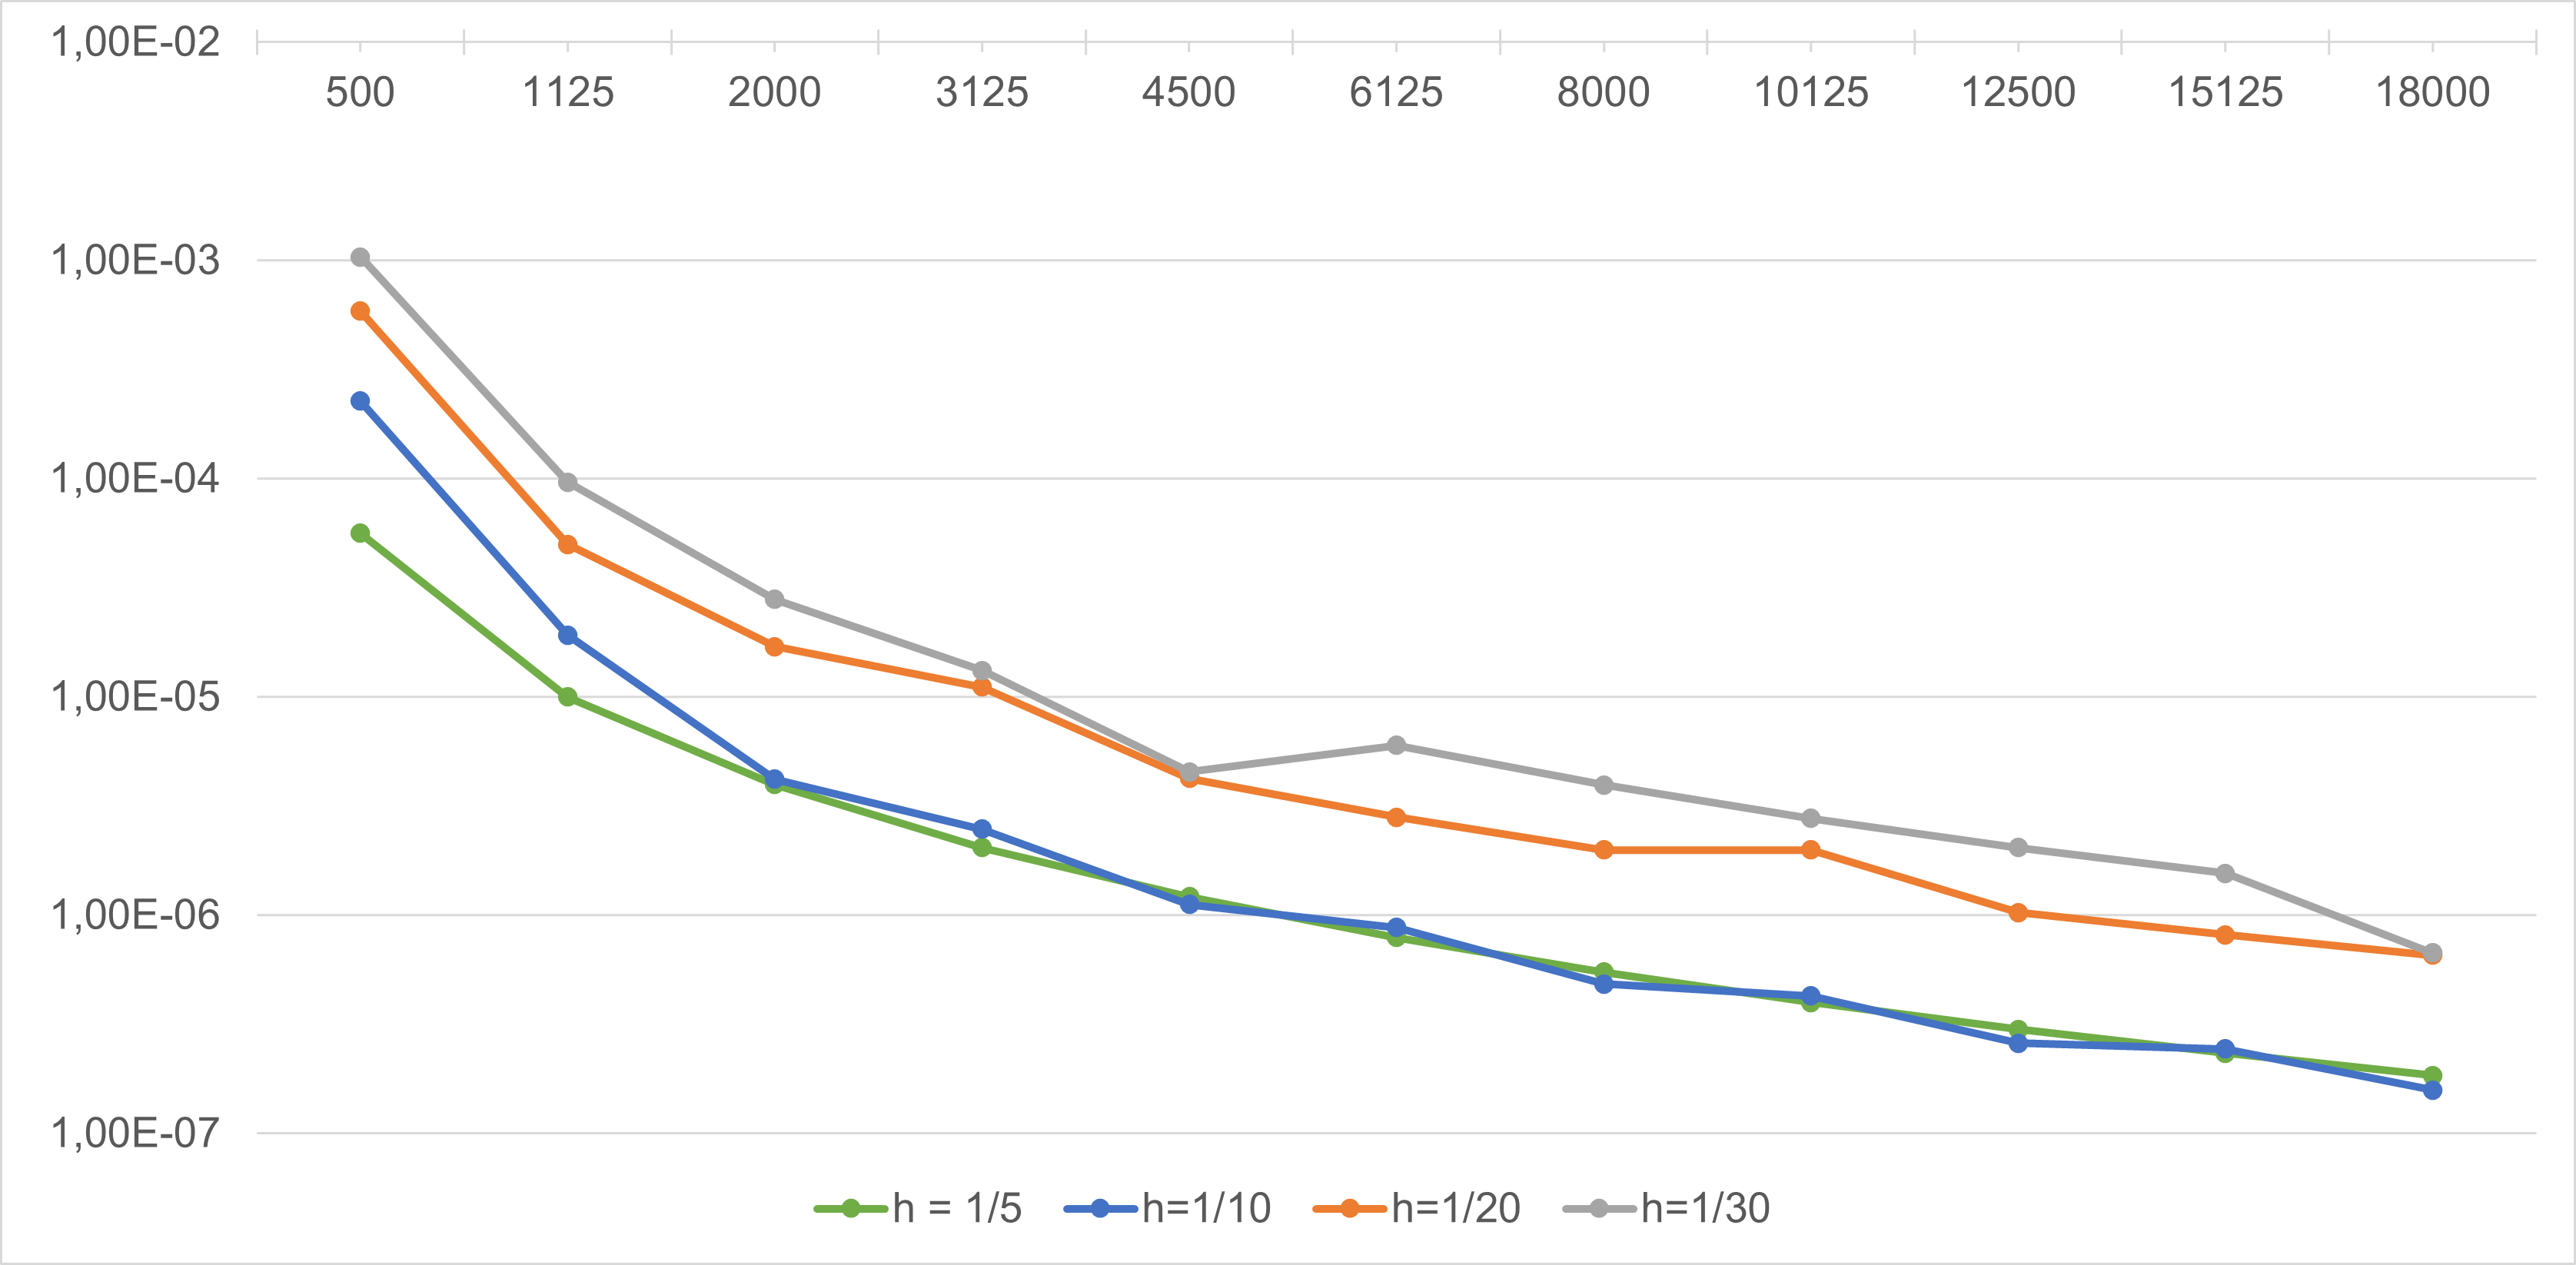
\includegraphics[scale=0.4]{Convergence.png}
			\caption{Maximum relative error of the first 10 eigenvalues of the two-dimensional beam.}
			\label{fig:conv}
		}
	\end{center}	
\end{figure}

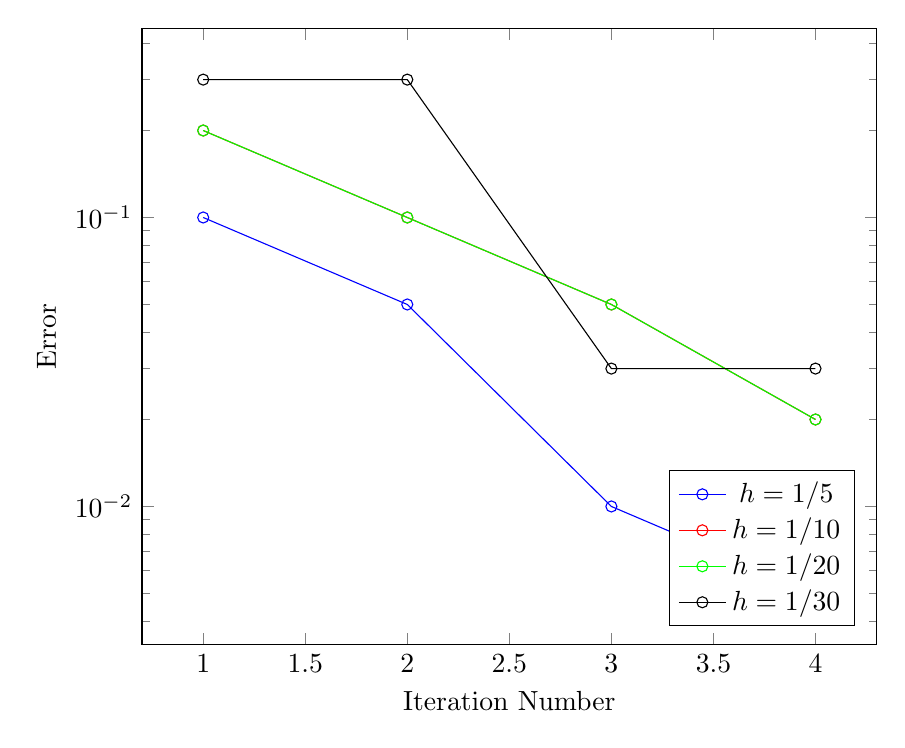
\begin{tikzpicture}
\begin{axis}[width=0.9\textwidth,
			 xlabel=Iteration Number,
			 ylabel=Error,
			 ymode=log,
			 legend pos=south east]
\addplot[color=blue, mark=o] coordinates {
    (1,0.1)
    (2,0.05)
    (3,0.01)
    (4,0.005)
};
\addlegendentry{$h=1/5$}

\addplot[color=red, mark=o] coordinates {
    (1,0.2)
    (2,0.1)
    (3,0.05)
    (4,0.02)
};
\addlegendentry{$h=1/10$}

\addplot[color=green, mark=o] coordinates {
    (1,0.2)
    (2,0.1)
    (3,0.05)
    (4,0.02)
};
\addlegendentry{$h=1/20$}

\addplot[color=black, mark=o] coordinates {
    (1,0.3)
    (2,0.3)
    (3,0.03)
    (4,0.03)
};
\addlegendentry{$h=1/30$}

\end{axis}
\end{tikzpicture}


Figure \ref{fig:conv} show the maximum relative error of the first 10 eigenvalues of the two-dimensional beam. In \cite{LVV09}, the authors use a grid size of $40 \times 10$ with $h= 1/10$ (or $\alpha = 1200$) and $h = 1/5$ (or $\alpha = 300$).\\

 Figure \ref{fig:conv} show that this can be improved significantly. For each case of $h$, the grid size is calculated as $n \times \max\left\{\lceil\frac{n}{h}\rceil,10\right\}$. This ensures that the nodes are distributed somewhat evenly relative to the length-width ratio. For this chapter, the results of the Timoshenko beam and two-dimensional beam are given accurate up to 5 significant digits.

\subsection{Comparing the shape of the eigenfunctions}
Before the eigenvalues can be compared, a method is required to be able to match the eigenvalues of the two different models. The authors of \cite{LVV09} match the modal shapes of the eigenfunctions. The corresponding eigenvalues can then be matched.\\

The eigenvalues of the Timoshenko beam, are referred to by the authors as beam-type eigenvalues.

\subsubsection{Shapes relating to beam-type eigenvalues}
The following figures are examples of beam-type mode shapes for the displacement $w$.

\begin{figure}[h!]
	\scalebox{.8}{
		\makebox[\textwidth][c]{
			\centering
			\begin{minipage}[b]{0.8\linewidth}
				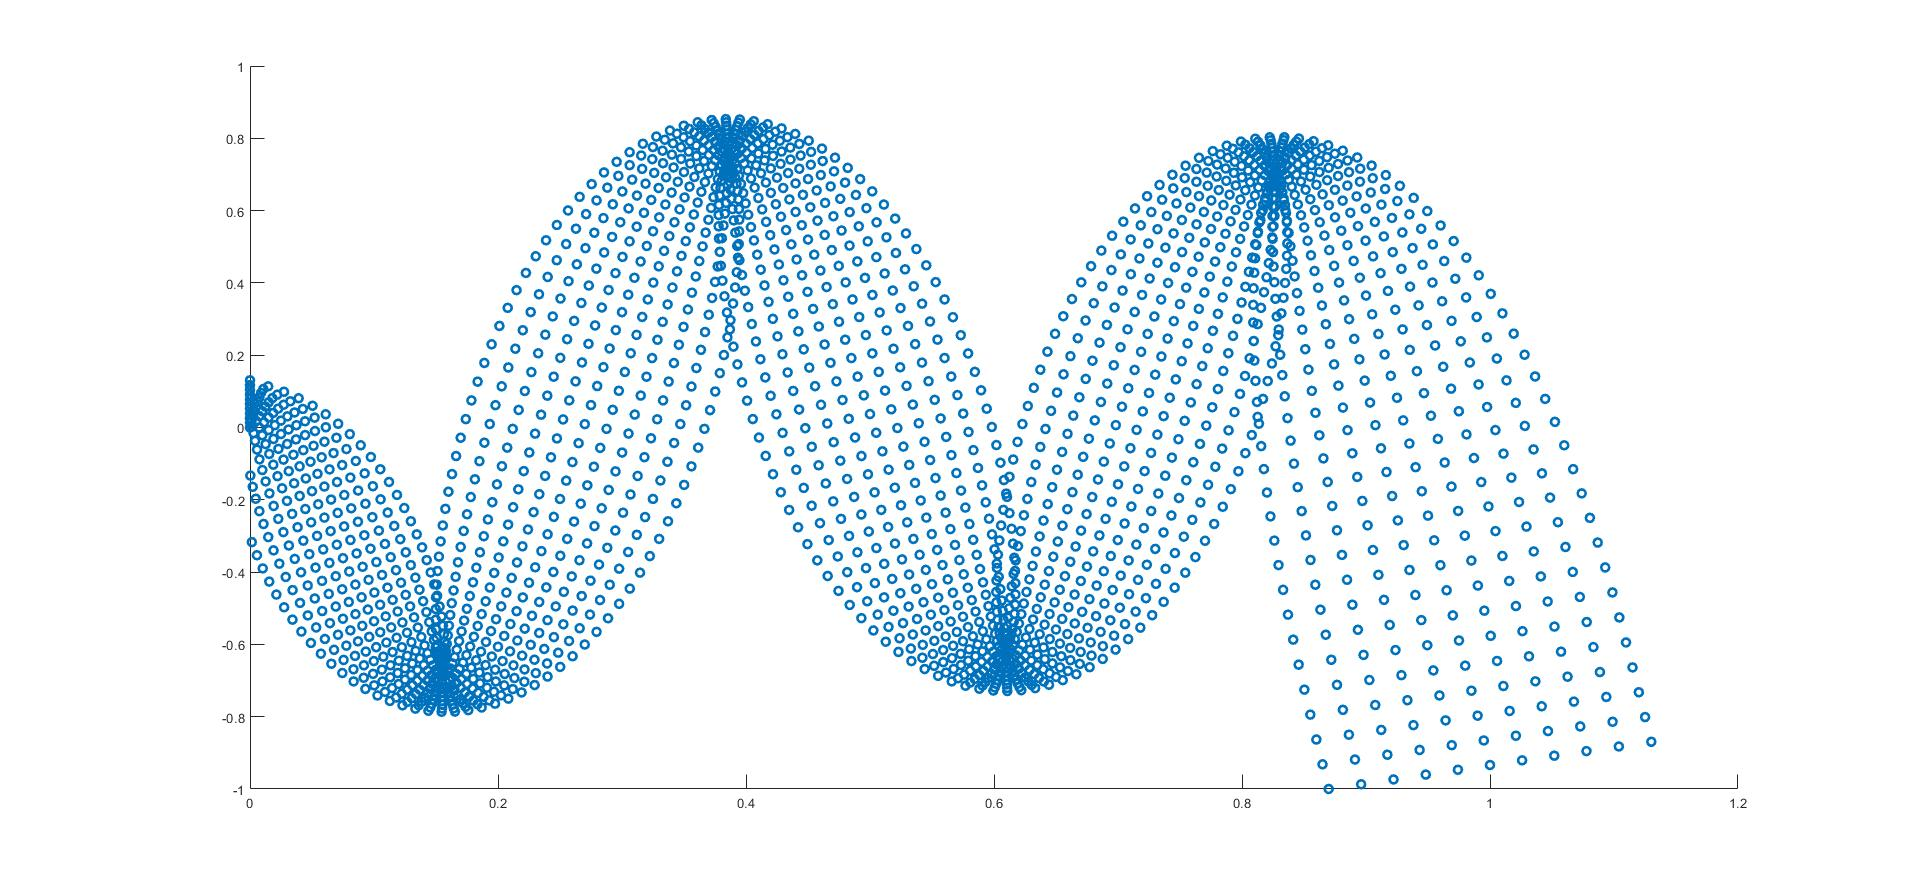
\includegraphics[width=1\linewidth]{Beam1.jpg}
				\subcaption{2D Beam Type - $\lambda_6 = 21.911$}
				\label{fig:minipage2}
			\end{minipage}
			\begin{minipage}[b]{0.8\linewidth}
				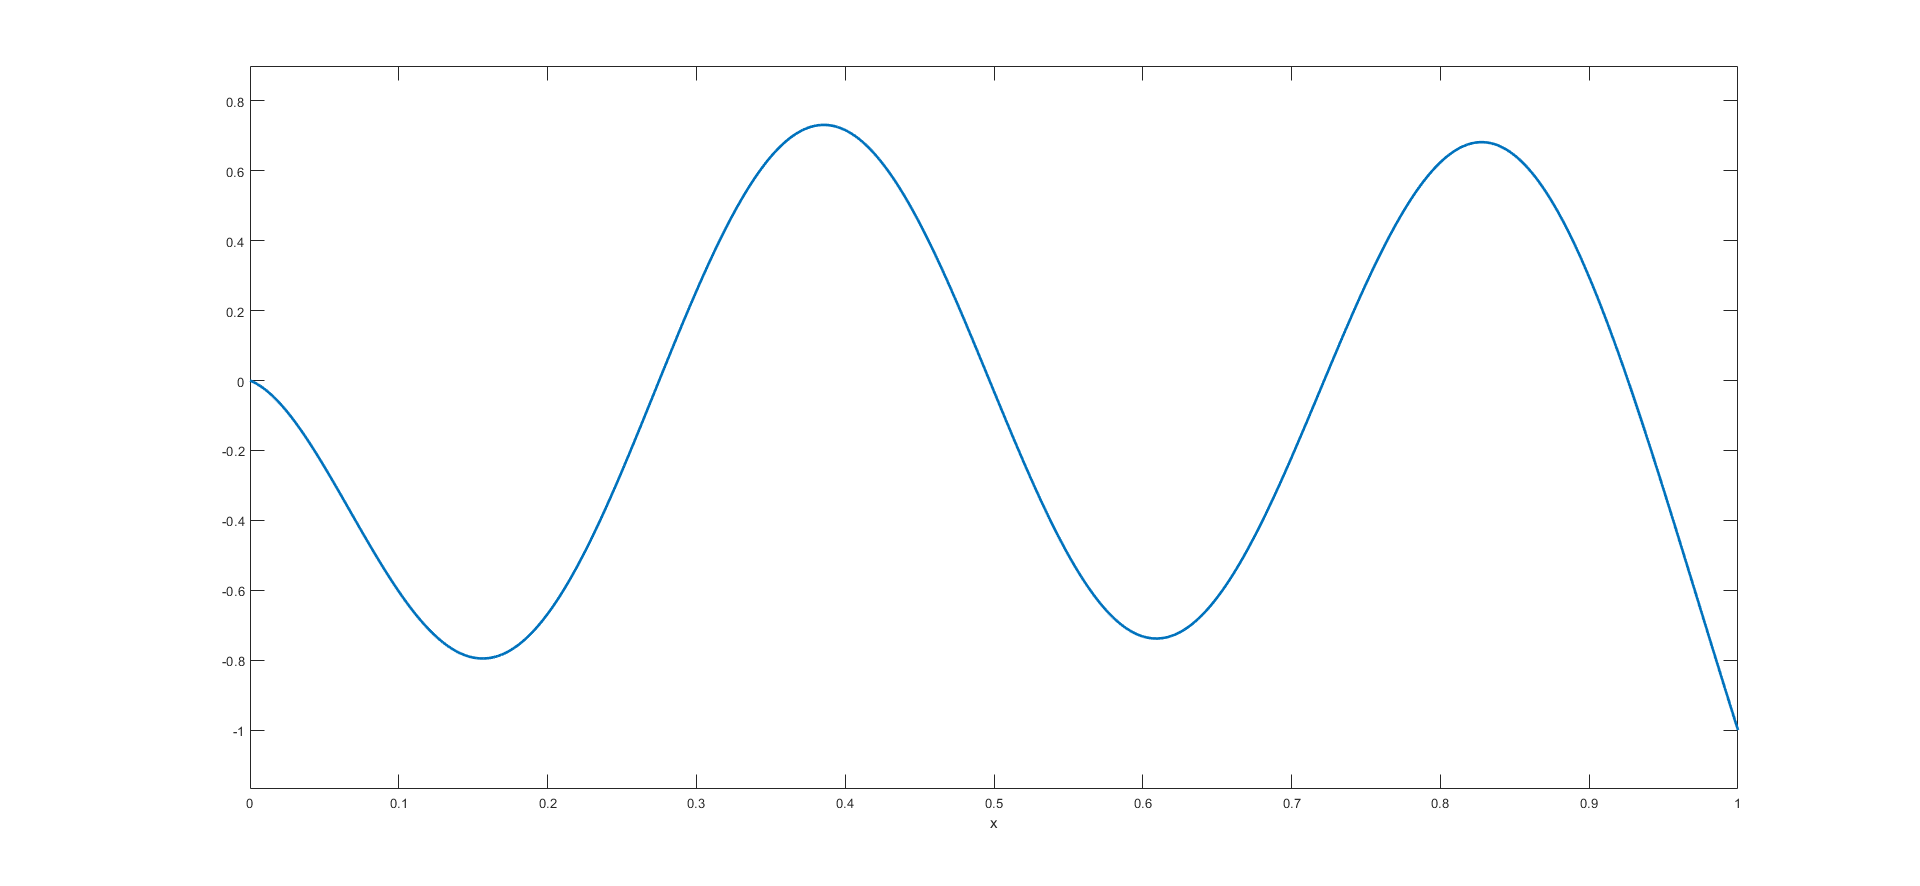
\includegraphics[width=1\linewidth]{1DBeam2.png}
				\subcaption{Timoshenko - $\lambda_5 = 21.794$}
				\label{fig:minipage1}
			\end{minipage}
	}}
	\scalebox{.8}{
		\makebox[\textwidth][c]{
			\begin{minipage}[b]{0.8\linewidth}
				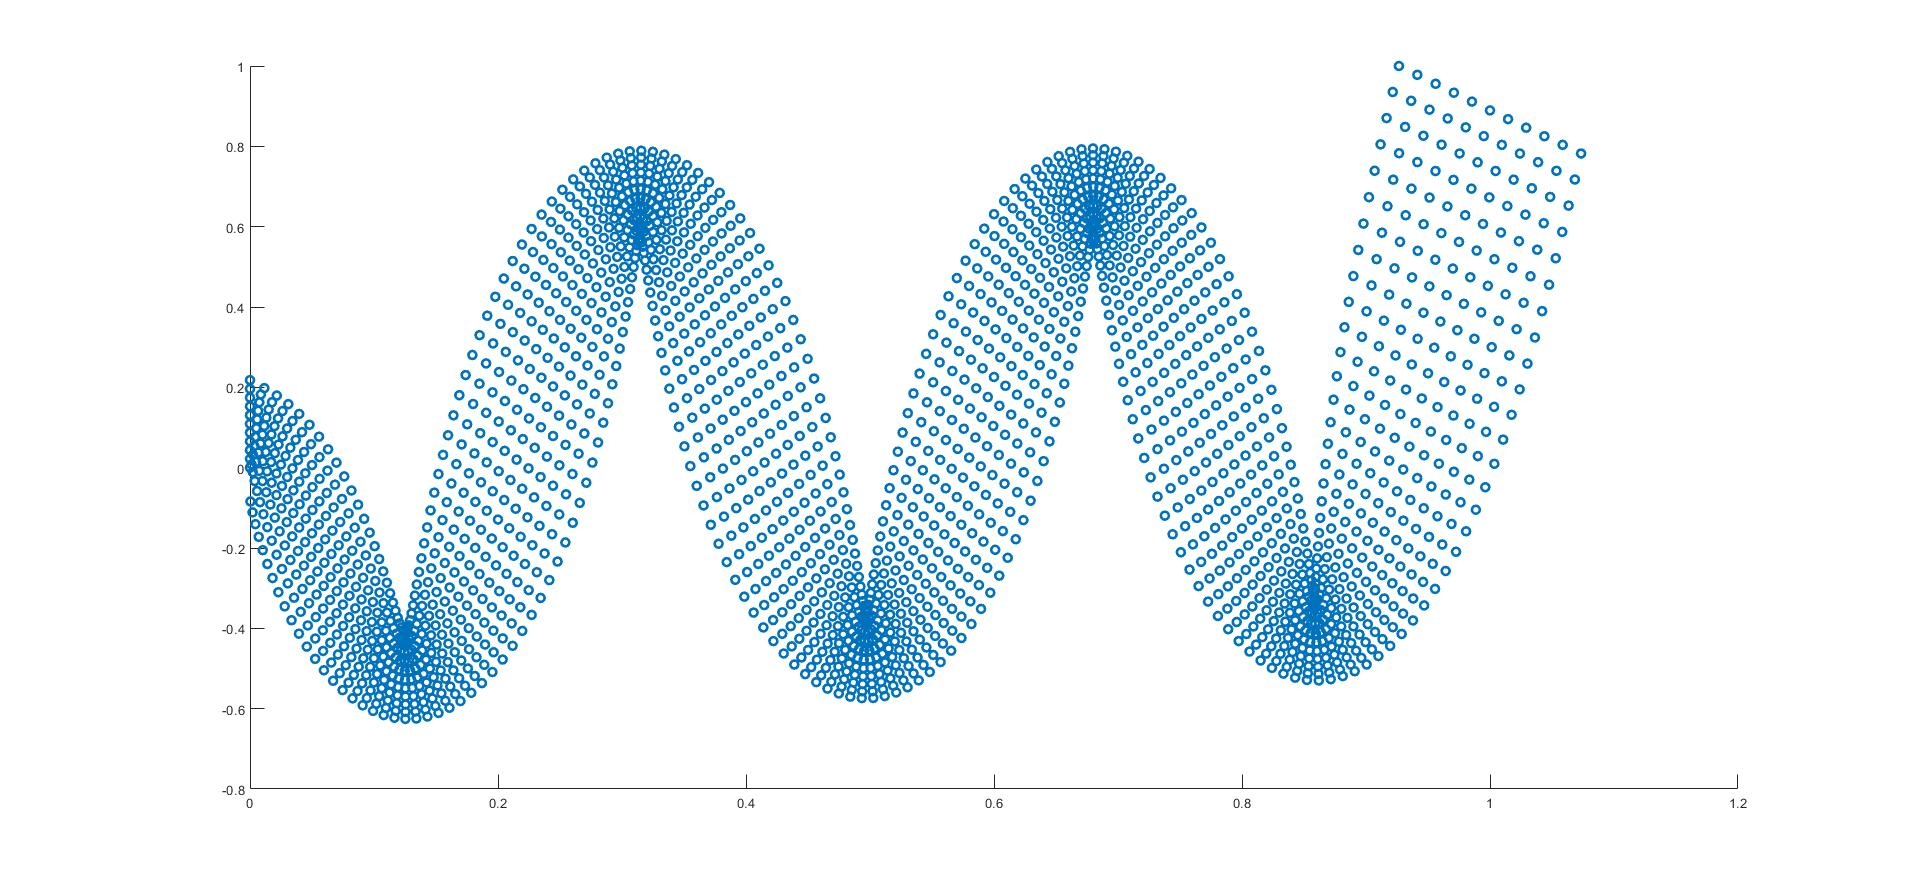
\includegraphics[width=1\linewidth]{Beam2.jpg}
				\subcaption{2D Beam Type - $\lambda_7 = 45.711$}
				\label{fig:minipage2}
			\end{minipage}
			\begin{minipage}[b]{0.8\linewidth}
				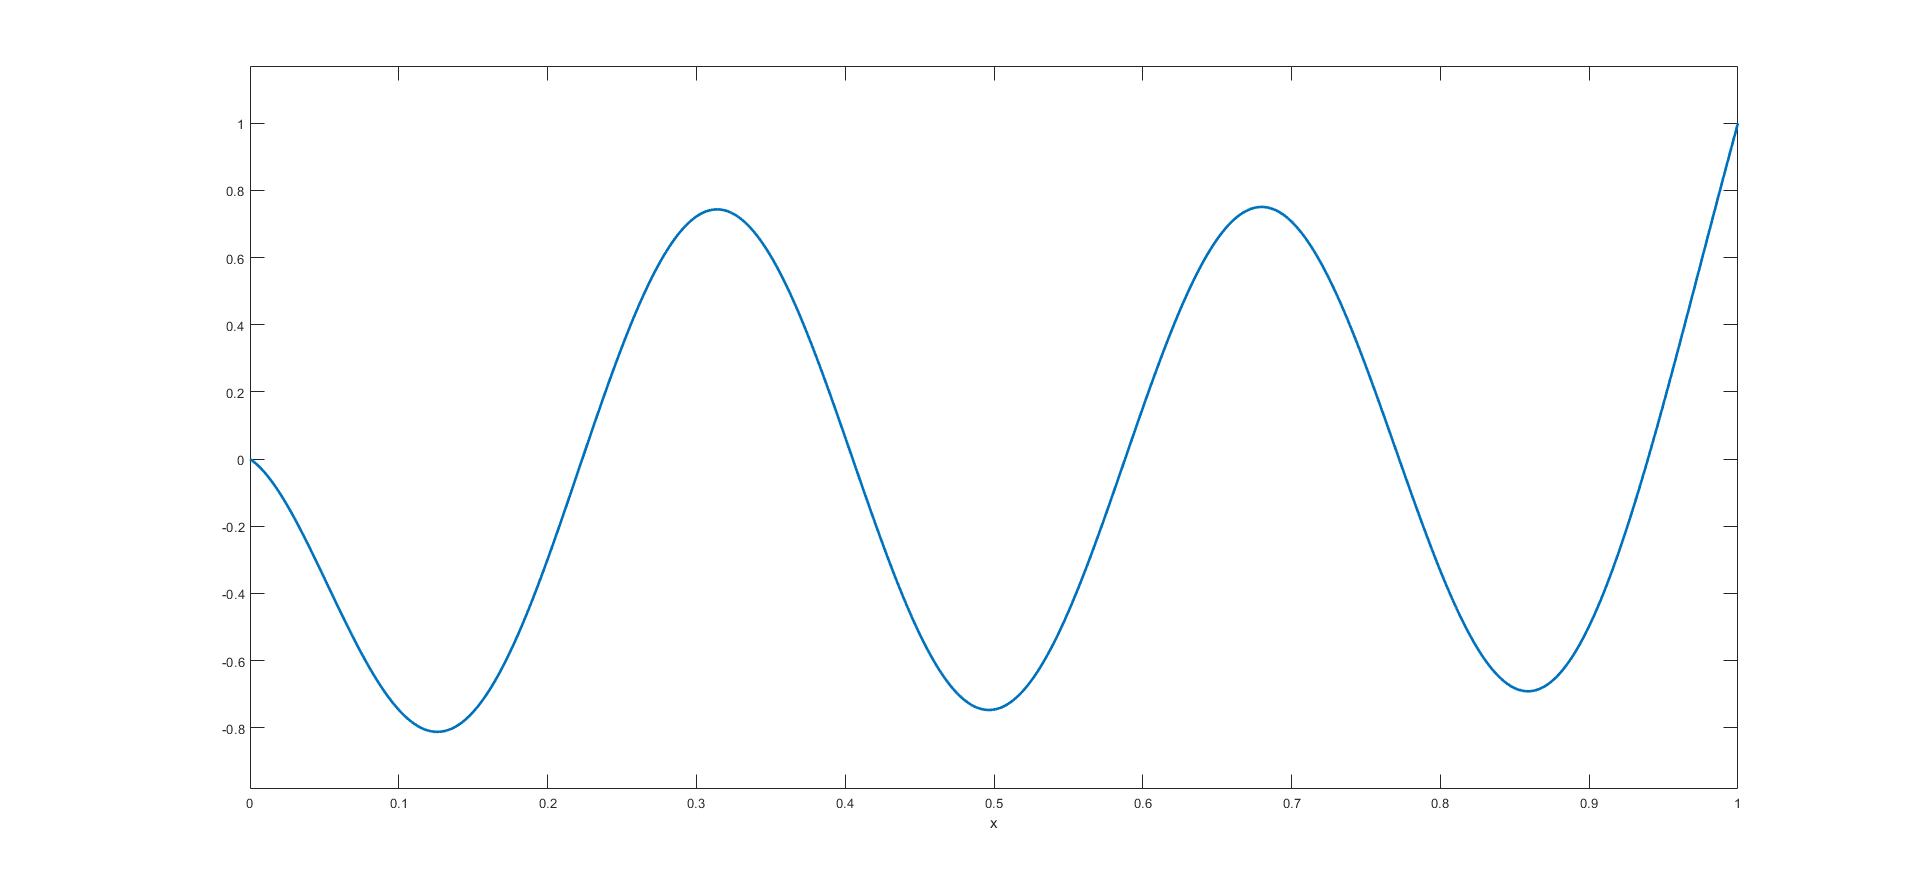
\includegraphics[width=1\linewidth]{1DBeam1.png}
				\subcaption{Timoshenko - $\lambda_6 = 45.390$}
				\label{fig:minipage1}
			\end{minipage}
			\caption{Modal shapes of the displacement $w$ for the beam-type 2D body and the Timoshenko beam with $\alpha = 4800$ ($h = 1/20$).}
		}
	}
\end{figure}
\FloatBarrier

\subsubsection{Shapes relating to non-beam type eigenvalues}
The following figures are examples of non beam-type mode shapes for the displacement $w$. These mode shapes are not present in the cantilever Timoshenko beam model and are not beam related. 
\begin{figure}[h!]
	\scalebox{.8}{
		\makebox[\textwidth][c]{
			\centering
			\begin{minipage}[b]{0.8\linewidth}
				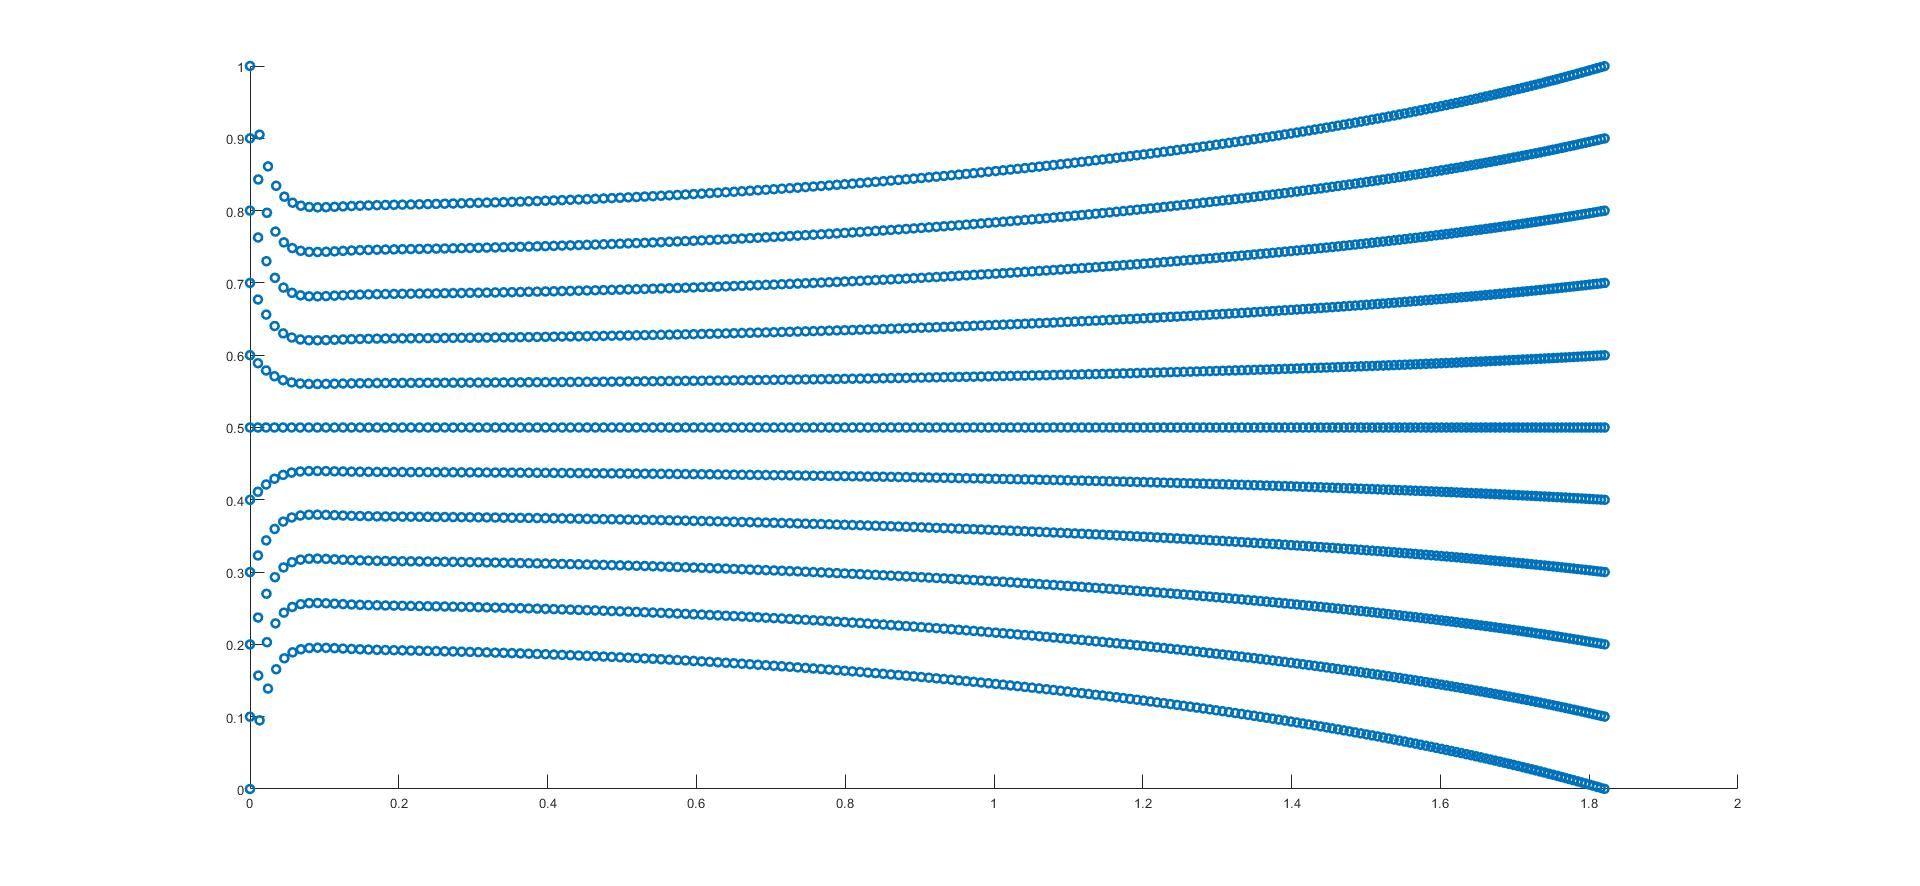
\includegraphics[width=1\linewidth]{NotBeam1.jpg}
				\subcaption{Non-Beam Type - $\lambda_4 = 7.7077$}
				\label{fig:minipage2}
			\end{minipage}
			\begin{minipage}[b]{0.8\linewidth}
				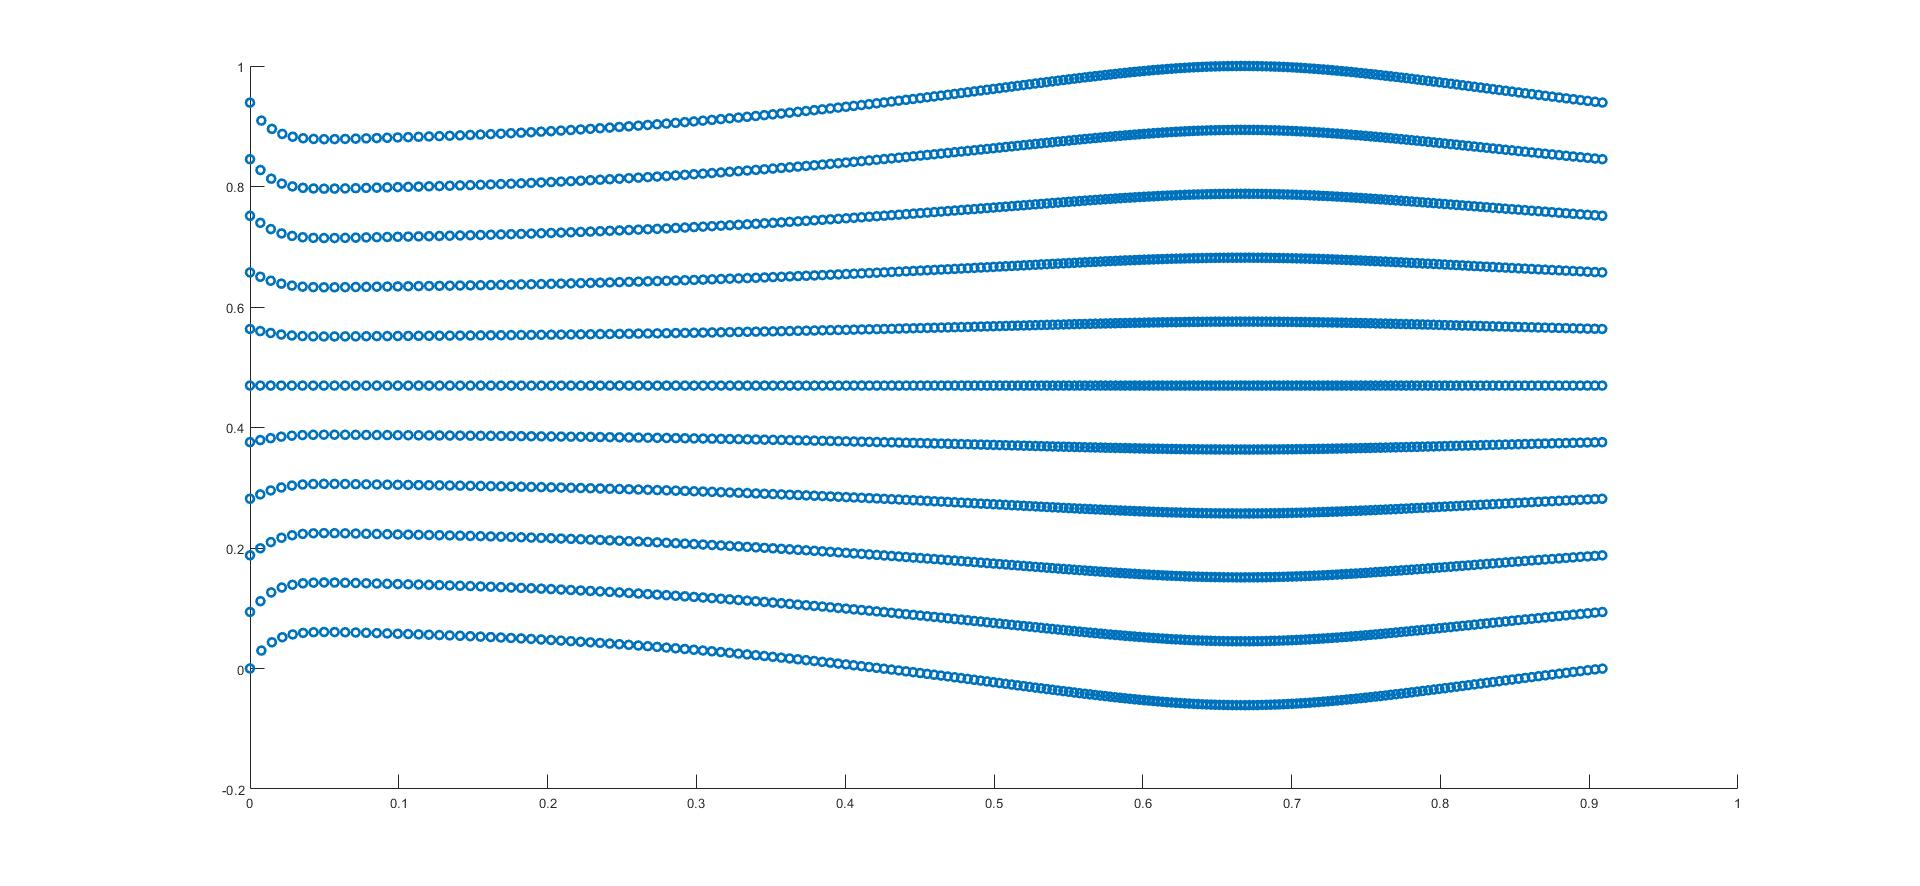
\includegraphics[width=1\linewidth]{NotBeam2.jpg}
				\subcaption{Non-Beam Type - $\lambda_8 = 69.344$}
				\label{fig:minipage1}
			\end{minipage}
			\caption{Modal shapes of the displacement $w$ for the non-beam type 2D body with $h = 1/20$.}
		}
	}
\end{figure}
\FloatBarrier

The existence of these non-beam type eigenvalues imply that there are eigenvalues in the two-dimensional model, that are not in the Timoshenko beam model. This is an example of the complexities that arise when comparing models of different dimensions.

\subsubsection{Shapes of the cross-section}
The Timoshenko beam theory improve some one-dimensional beam theories such as the Euler-Bernoulli beam theory by also including the effect of shear. In the Timoshenko beam theory it is assumed that the cross-sections need not remain perpendicular to the neutral axis of the beam. The cross-sections however remain a straight line.\\

For the two-dimensional beam, the shape of the cross-section can deform into a s-shape. This is explained in \cite{LVV09} and a similar figure in \cite{LVV09} is given here.
\FloatBarrier
\begin{figure}[h!]
	\centering
	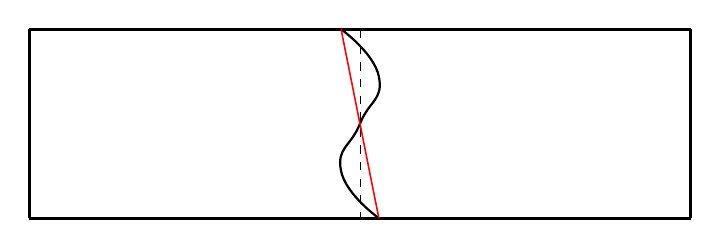
\begin{tikzpicture}[scale=1.2]
	
	\draw[line width = 0.4mm] (0,1) -- (7,1);
	\draw[line width = 0.4mm] (0,-1) -- (7,-1);
	\draw[line width = 0.4mm] (7,-1) -- (7,1);
	\draw[line width = 0.4mm] (0,-1) -- (0,1);
	
	
	\draw[line width = 0.1mm,dashed] (3.5,1) -- (3.5,-1);
	
	\draw[thick] plot [smooth,tension=0.9] coordinates{(3.3,1) (3.7,0.5) (3.5,0) (3.3,-0.5) (3.7,-1)};
	
	\draw[line width = 0.2mm,red] (3.3,1) -- (3.7,-1);
	
\end{tikzpicture}
	\caption{S-shape deformation of the cross-section.}\label{fig:s}
\end{figure}

Note that figure \ref{fig:s} shows an exaggerated example of the deformation of a cross-section. The red line shows how the average rotation of a cross-section is calculated in \cite{LVV09}. This average rotation can be used to compare the rotation of the cross-section of the two-dimensional beam to the rotation of the cross-section of the Timoshenko beam.
\FloatBarrier

\subsubsection{Direct comparison of mode shapes}
Figure \ref{fig:w} shows the displacement of the material lines of the cantilever Timoshenko beam and the cantilever two-dimensional beam, compared directly.

\begin{figure}[ht!]
	\scalebox{.8}{
		\makebox[\textwidth]{
			\centering
			\centering
			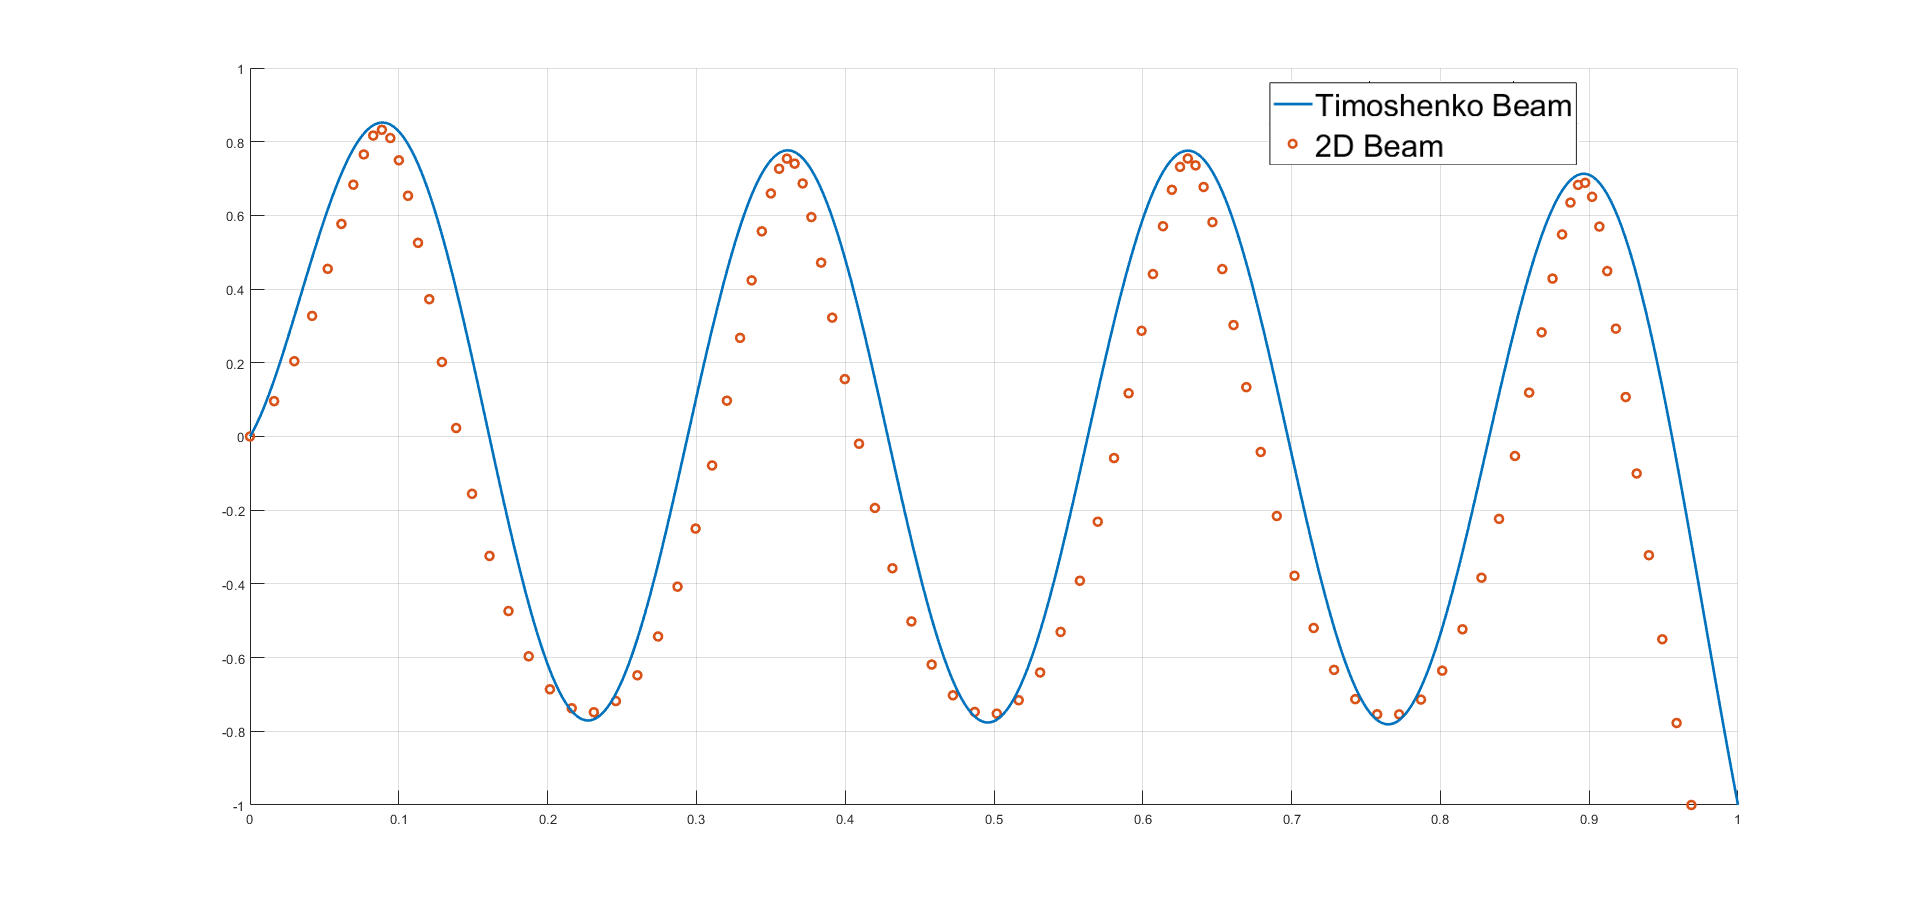
\includegraphics[scale=0.4]{1Dv2D.png}
			\caption{Comparison of the displacement $w$ mode shape corresponding to $\lambda_{10}$ for the 2D beam and $\lambda_8$ for the Timoshenko beam with $\alpha = 4800$ ($h=1/20$)}
			\label{fig:w}}}
\end{figure}
\FloatBarrier

Similarly Figure \ref{fig:phi} shows the direct comparison of the angle of the cross-section of the cantilever Timoshenko beam and the two-dimensional beam. The average rotation of the cross-section of the two-dimensional beam's mode shape is calculated as shown in figure \ref{fig:s} and \cite{LVV09}.

\FloatBarrier
\begin{figure}[ht!]
	\scalebox{.8}{
		\makebox[\textwidth]{
			\centering
			\centering
			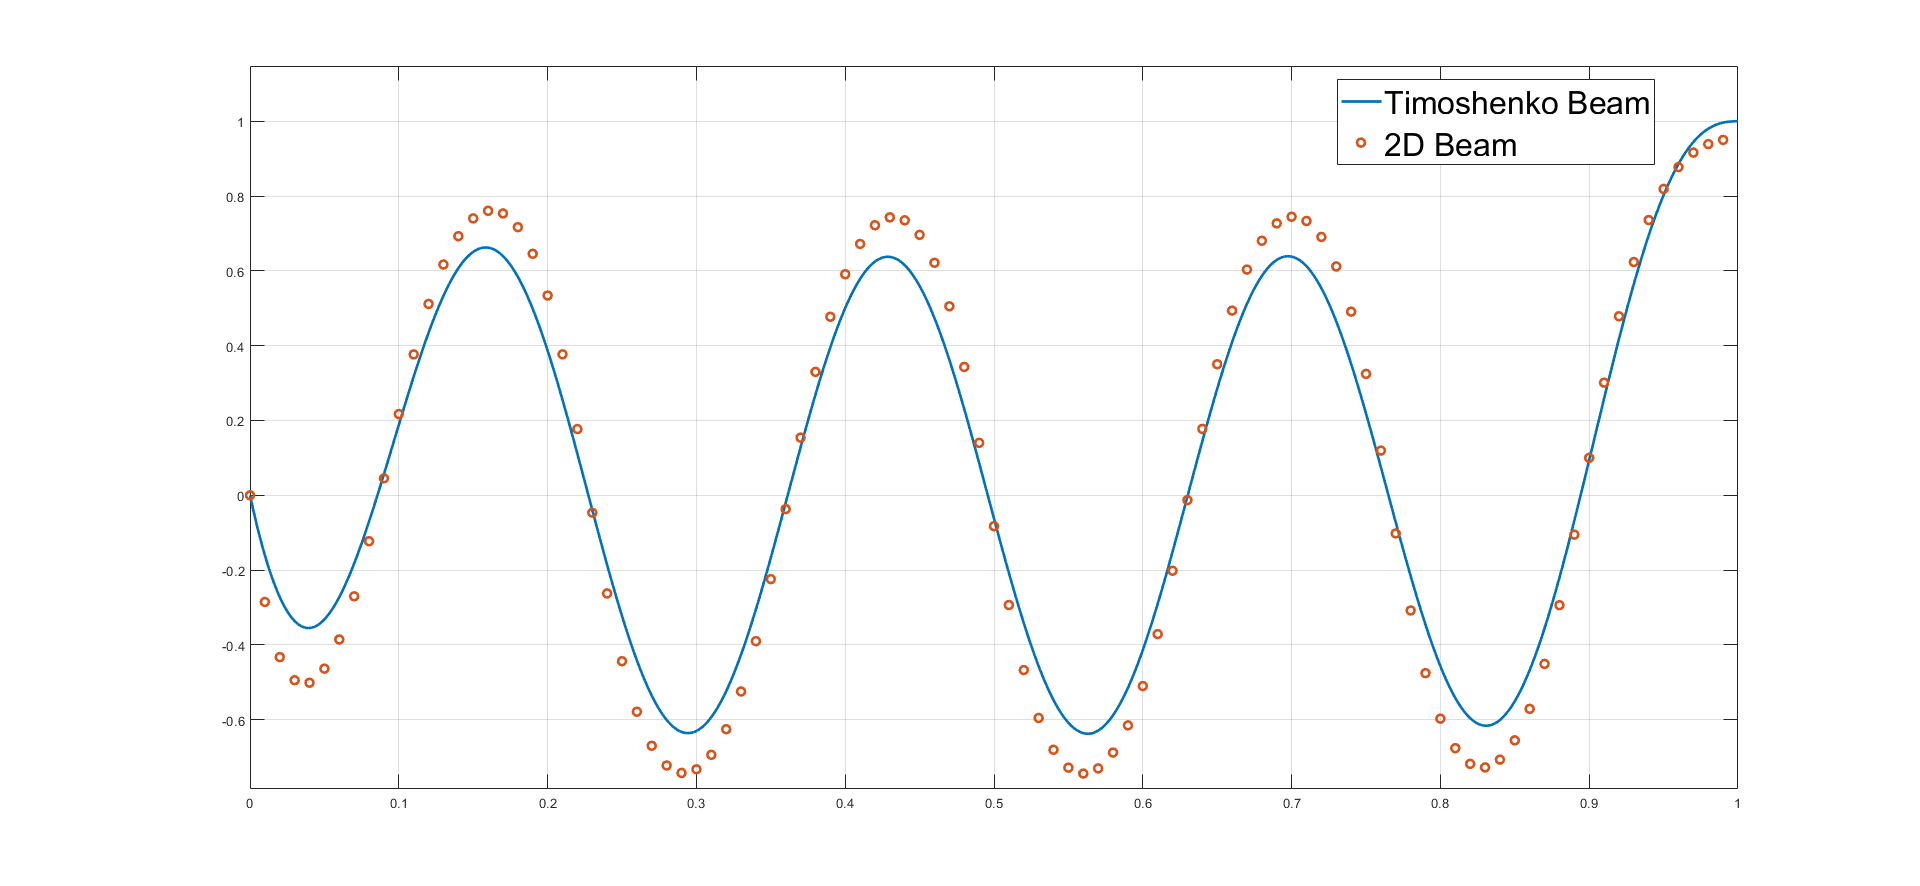
\includegraphics[scale=0.4]{1Dv2Dphi.png}
			\caption{Comparison of the angle $\phi$ (best fit for 2D Beam) mode shape corresponding to $\lambda_{10}$ for the 2D beam and $\lambda_8$ for the Timoshenko beam with $\alpha = 4800$ ($h=1/20$)}
			\label{fig:phi}}}
\end{figure}
\FloatBarrier

In \cite{LVV09} the authors obtained similar results for $\alpha=300$, which represents a short beam. Both figures \ref{fig:w} and \ref{fig:phi} were calculated with5 $\alpha = 4800$, which represents a longer, narrower beam. 

\subsubsection{Remark}
The mode shapes were scaled to obtain figures \ref{fig:w} and \ref{fig:phi}. Therefore no scale is shown on the y-axis.

\subsection{Comparing the eigenvalues}
\subsubsection{Results of [LVV09]}
The following table contains the results form \cite{LVV09} as well as the corresponding results obtained in this dissertation.
\begin{table}[!ht]
	\centering
	\caption{Results from [LVV09] and results obtained in this dissertation. $0^a$ indicates a 0 as a result of rounding. $\alpha = 1200$}
	\begin{tabular}{|c|c|c|c||c|c|c|c|}
		\hline
		\multicolumn{4}{|c||}{Results from [LVV09]} & \multicolumn{4}{c|}{Dissertation} \\ \hline \hline
		~ & 2D & Timo & RE & ~ & 2D & Timo & RE  \\ \hline
		1 & 0.0317 & 0.0316 & 0.00315 & 1 & 0.031713 & 0.031639 & 0.0023407  \\ 
		2 & 1.14 & 1.14 & $0^a$ & 2 & 1.1413 & 1.1365 &  0.0042050 \\ 
		3 & 7.72 & - & ~ & 3 & 7.7161 & - &   \\ 
		4 & 7.92 & 7.86 & 0.00758 & 4 & 7.918 & 7.8617 & 0.0071116    \\ 
		5 & 26.2 & 25.9 & 0.0115 & 5 & 26.148 & 25.869 & 0.010669  \\ 
		6 & 60.8 & 59.9 & 0.0148 & 6 & 60.816 & 59.946 & 0.014303  \\ 
		7 & 69.3 & - & ~ & 7 & 69.344 & - &    \\ 
		8 & 115 & 113 & 0.0174 & 8 & 115.28 & 113.23 &  0.017787  \\ 
		9 & 192 & 188 & 0.0208 & 9 & 191.57 & 187.55 &  0.020999  \\ 
		10 & 192 & - &  & 10 & 192.03 & - &   \\ 
		11 & 291 & 284 & 0.0241 & 11 & 290.76 & 283.81 &  0.023899  \\ \hline
	\end{tabular}\label{Results_LVV09}
\end{table}

In Table \ref{Results_LVV09}, the results from \cite{LVV09} and the respective results from this dissertation is given. This table shows that the results of \cite{LVV09} can be replicated with more significant digits.\\

Interestingly, with the improved accuracy over \cite{LVV09}, the relative errors remain similar in Table \ref{Results_LVV09}. It is possible that the higher level of accuracy will only benefit larger eigenvalues. Larger eigenvalues are however not of interest for practical applications. The 2nd relative error of \cite{LVV09} however could not be duplicated.

\subsection{Comparison of the eigenvalues}
In \cite{LVV09}, two values for $\alpha$ are considered. For $\alpha = 1200$, the Timoshenko beam has a length to width ratio of $1:10$. For $\alpha = 300$, the Timoshenko beam has length to width ratio of $1:5$. These two values represent a ``long slender'' beam and a ``short'' beam.\\

In Table \ref{tab:Timo}, the eigenvalues of the Timoshenko beam are compared to the first 20 eigenvalues of the two-dimensional beam. The eigenvalues are calculated for different values of $\alpha$.\\

\begin{table}[h!]
	\scalebox{.8}{
	\makebox[\textwidth]{
	\caption{Eigenvalues of a Timoshenko cantilever beam vs the eigenvalues of a cantilever two-dimensional elastic body. RE - Relative Error}
	\begin{tabular}{|cccc||cccc||cccc||cccc|}
		\hline
		\multicolumn{16}{|c|}{Comparison of Eigenvalues} \\
		\hline\hline
		\multicolumn{4}{|c||}{ $h = 1/5$ or $\alpha = 300$}       & \multicolumn{4}{c||}{$h =1/10$ or $\alpha = 1200$}      & \multicolumn{4}{c||}{$h = 1/20$ or $\alpha = 4800$}      & \multicolumn{4}{c|}{$h = 1/30$ or $\alpha = 10800$} \\
		\hline
		{i} & {2D} & {j} & {Timo} & {i} & {2D} & {j} & {Timo} & {i} & {2D} & {j} & {Timo} & {i} & {2D} & {j} & {Timo} \\
		\hline
		{1}&0.12151&1&0.12092&1&0.031713&1&0.031639&1&0.008013&1&0.008004&1&0.003568&1&0.003565\\
		{2}&3.5460&2&3.5071&2&1.1413&2     & 1.1365 & 2     & 0.30756 & 2     & 0.30705 & 2     & 0.13869 & 2     & 0.13855 \\
		\cellcolor{lightgray}{3} & \cellcolor{lightgray}{7.7311} &       & {-} & \cellcolor{lightgray}{3}     & \cellcolor{lightgray}{7.7161} &       & {-} & 3     & 2.3273 & 3     & 2.3213 & 3     & 1.0698 & 3     & 1.0683 \\
		{4} & 20.225 & 3     & 19.869 & 4     & 7.9180 & 3     & 7.8617 & \cellcolor{lightgray}{4}     & \cellcolor{lightgray}{7.7077} &       & {-} & 4     & 4.0140 & 4     & 4.0058 \\
		{5} & 56.109 & 4     & 54.766 & 5     & 26.148 & 4     & 25.869 & 5     & 8.5086 & 4     & 8.4762 & \cellcolor{lightgray}{5}     & \cellcolor{lightgray}{7.7047} &       & {-} \\
		\cellcolor{lightgray}{6} & \cellcolor{lightgray}{69.164} &       & {-} & 6     & 60.816 & 5     & 59.946 & 6     & 21.911 & 5     & 21.794 & 6     & 10.655 & 5     & 10.625 \\
		{7} & 114.03 & 5     & 110.75 & \cellcolor{lightgray}{7}     & \cellcolor{lightgray}{69.344} &       & {-} & 7     & 45.711 & 6     & 45.390 & 7     & 22.975 & 6     & 22.890 \\
		{8} & {189.17} &  6     & {186.50} & 8     & 115.28 & 6     & 113.23 & \cellcolor{lightgray}{8}     & \cellcolor{lightgray}{69.344} &       & {-} & 8     & 43.113 & 7     & 42.909 \\
		\cellcolor{lightgray}{9} & \cellcolor{lightgray}{192.61} &      &  & {9}     & {191.57} &   7  & {187.55} & 9     & 82.887 & 7     & 82.154 & \cellcolor{lightgray}{9}     & \cellcolor{lightgray}{69.331} &       & {-} \\
		{10} & 285.85 & 7     & 277.64 & \cellcolor{lightgray}{10}    & \cellcolor{lightgray}{192.03} &      & {-} & 10    & 136.03 & 8     & 134.58 & 10    & 73.230 & 8     & 72.803 \\
		{11} & 328.40 & 8     & 330.29 & 11    & 290.76 & 8     & 283.81 & \cellcolor{lightgray}{11}    & \cellcolor{lightgray}{192.48} &       & {-} & 11    & 115.41 & 9     & 114.61 \\
		\cellcolor{lightgray}{12} & \cellcolor{lightgray}{357.08} &       & {-} & \cellcolor{lightgray}{12}    & \cellcolor{lightgray}{374.45} &       & {-} & 12    & 207.29 & 9     & 204.69 & 12    & 171.61 & 10    & 170.20 \\
		{13} & 397.33 & 9     & 394.02 & 13    & 413.20 & 9     & 402.27 & 13    & 298.38 & 10    & 294.10 & \cellcolor{lightgray}{13}    & \cellcolor{lightgray}{192.52} &       & {-} \\
		{14} & 442.00   & 10    & 439.52 & 14    & 558.67 & 10    & 542.65 & \cellcolor{lightgray}{14}    & \cellcolor{lightgray}{376.83} &       & {-} & 14    & 243.56 & 11    & 241.26 \\
		\cellcolor{lightgray}{15} & \cellcolor{lightgray}{533.71} &       & {-} & \cellcolor{lightgray}{15}    & \cellcolor{lightgray}{614.11} &       & {-} & 15    & 410.63 & 11    & 404.01 & 15    & 332.83 & 12    & 329.28 \\
		{16} & 538.97 & 11    & 541.55 & 16    & 726.26 & 11    & 704.15 & 16    & 545.03 & 12    & 535.32 & \cellcolor{lightgray}{16}    & \cellcolor{lightgray}{377.16} &       & {-} \\
		\cellcolor{lightgray}{17} & \cellcolor{lightgray}{596.06} &       & {-} & \cellcolor{lightgray}{17}    & \cellcolor{lightgray}{906.28} &       & {-} & \cellcolor{lightgray}{17}    & \cellcolor{lightgray}{621.95} &       & {-} & 17    & 440.77 & 13    & 435.51 \\
		{18} & 602.77 & 12    & 596.09 & 18    & 913.69 & 12    & 884.92 & 18    & 702.30 & 13    & 688.64 & 18    & 568.51 & 14    & 561.04 \\
		\cellcolor{lightgray}{19} & \cellcolor{lightgray}{657.87} &       & {-} & 19    & 1113.7 & 13    & 1080.1 & 19    & 882.95 & 14    & 864.40 & \cellcolor{lightgray}{19}    & \cellcolor{lightgray}{623.05} &       & {-} \\
		{20} & 717.37 & 13    & 731.74 & \cellcolor{lightgray}{20}    & \cellcolor{lightgray}{1218.0}  &       & {-} & \cellcolor{lightgray}{20}    & \cellcolor{lightgray}{927.18} &       & {-} & 20    & 717.04 & 15    & 706.74 \\
		\hline
		\multicolumn{2}{|c}{Max RE:} & \multicolumn{2}{c||}{3.1718\%} & \multicolumn{2}{c}{Max RE:} & \multicolumn{2}{c||}{3.1486\%} & \multicolumn{2}{c}{Max RE:} & \multicolumn{2}{c||}{2.1018\%} & \multicolumn{2}{c}{Max RE:} & \multicolumn{2}{c|}{1.4361\%} \\
		\hline
	\end{tabular}%
	\label{tab:Timo}%
}
}
\end{table}%
\FloatBarrier

The authors of \cite{LVV09} show that for $\alpha = 300$ the eigenvalues compare very well up to the 20th two-dimensional eigenvalue. This is also apparent for other values of $\alpha$ as Table \ref{tab:Timo} shows. In fact, the accuracy of the eigenvalues increases as $\alpha$ increases. The authors of \cite{LVV09} also mention that for $\alpha = 100$, the results are very good for the first 10 eigenvalues.\\

Interestingly, the number of non-beam type eigenvalues within the first few eigenvalues decreases as $\alpha$ increases (or more relevant for the two-dimensional beam: as $h$ decreases).\\

Overall, the relevant conclusions of \cite{LVV09} is verified. For practical applications of beam models, the Timoshenko beam can be used. Preferably for long slender beams as Table \ref{tab:Timo} shows. The authors also mention that nature of the disturbance should also be taken into consideration, mainly because the models are linear.\\

 The short comings of \cite{LVV09} is that damping is not considered. This is mentioned by the authors of \cite{LVV09}, but will not be addressed in this dissertation. Further work is to extend \cite{LVV09} to a three-dimensional comparison. This is investigated further in this chapter.\\

\section{Validity of the two-dimensional elastic model}
In this section, the validity of a two-dimensional cantilever beam is investigated. This is a natural extension of the work in \cite{LVV09}. This was mentioned by the authors.\\

As mentioned before, the two-dimensional model is used as a intermediate step between the Timoshenko and three-dimensional beam. The same method as in \cite{LVV09} will be used to investigate the validity of the two-dimensional model.\\

The models for the two-dimensional and three-dimensional beams are defined in section \ref{ssec:2D_Model:ModelProblem} and \ref{ssec:3D_Model:ModelProblems} respectively. These models are elastic bodies and not specifically beam models. Therefore it is expected to find eigenvalue and eigenfunction pairs that does not relate to beam type problems. This was already seen with the two-dimensional model in the previous section. These not beam type eigenvalues are calculated in this section, however the focus still remains on beam type problems.\\

\subsection{The models}
Recall a cantilever two-dimensional beam, referred to as Problem 2D-1 in section \ref{ssec:2D_Model:ModelProblem} and a cantilever three-dimensional beam, referred to as Problem 3D-1 in section \ref{ssec:3D_Model:ModelProblems}.\\

Figure \ref{fig:2Dv3D} shows the two beams side-by-side.

\FloatBarrier
\begin{figure}[h!]
	\scalebox{.8}{
		\makebox[\textwidth][c]{
			\caption{Side-by-side comparison of the beams.}
			\label{fig:2Dv3D}
			\centering
			\begin{minipage}[b]{0.7\linewidth}
				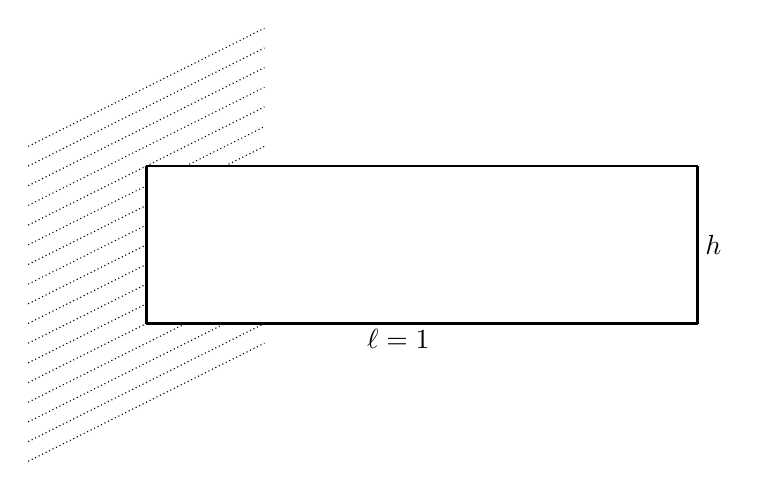
\begin{tikzpicture}
					\draw[line width = 0.3mm] (0,1) -- (7,1);
					\draw[line width = 0.3mm] (0,-1) -- (7,-1);
					\draw[line width = 0.3mm] (7,-1) -- (7,1);
					\draw[line width = 0.3mm] (0,-1) -- (0,1);
					
					
					\draw[scale=0.5, domain=-3:3, smooth, variable=\x,densely dotted] plot ({\x}, {0.5*\x+4});
					\draw[scale=0.5, domain=-3:3, smooth, variable=\x,densely dotted] plot ({\x}, {0.5*\x+3.5});
					\draw[scale=0.5, domain=-3:3, smooth, variable=\x,densely dotted] plot ({\x}, {0.5*\x+3});
					\draw[scale=0.5, domain=-3:3, smooth, variable=\x,densely dotted] plot ({\x}, {0.5*\x+2.5});
					\draw[scale=0.5, domain=-3:3, smooth, variable=\x,densely dotted] plot ({\x}, {0.5*\x+2});
					
					\draw[scale=0.5, domain=-3:0, smooth, variable=\x,densely dotted] plot ({\x}, {0.5*\x+1.5});
					\draw[scale=0.5, domain=-3:0, smooth, variable=\x,densely dotted] plot ({\x}, {0.5*\x+1});
					
					
					\draw[scale=0.5, domain=1:3, smooth, variable=\x,densely dotted] plot ({\x}, {0.5*\x+1.5});
					\draw[scale=0.5, domain=2:3, smooth, variable=\x,densely dotted] plot ({\x}, {0.5*\x+1});
					
					\draw[scale=0.5, domain=-3:0, smooth, variable=\x,densely dotted] plot ({\x}, {0.5*\x+0.5});
					\draw[scale=0.5, domain=-3:0, smooth, variable=\x,densely dotted] plot ({\x}, {0.5*\x});
					\draw[scale=0.5, domain=-3:0, smooth, variable=\x,densely dotted] plot ({\x}, {0.5*\x-0.5});
					\draw[scale=0.5, domain=-3:0, smooth, variable=\x,densely dotted] plot ({\x}, {0.5*\x-1});
					\draw[scale=0.5, domain=-3:0, smooth, variable=\x,densely dotted] plot ({\x}, {0.5*\x-1.5});
					\draw[scale=0.5, domain=-3:0, smooth, variable=\x,densely dotted] plot ({\x}, {0.5*\x-2});
					\draw[scale=0.5, domain=-3:1, smooth, variable=\x,densely dotted] plot ({\x}, {0.5*\x-2.5});
					\draw[scale=0.5, domain=-3:2, smooth, variable=\x,densely dotted] plot ({\x}, {0.5*\x-3});
					\draw[scale=0.5, domain=-3:3, smooth, variable=\x,densely dotted] plot ({\x}, {0.5*\x-3.5});
					\draw[scale=0.5, domain=-3:3, smooth, variable=\x,densely dotted] plot ({\x}, {0.5*\x-4});
					
					\node at (7.2,0) {$h$};
					\node at (3.2,-1.2) {$\ell = 1$};
				\end{tikzpicture}
				\subcaption{Two-Dimensional Elastic Body}
			\end{minipage}
			\begin{minipage}[b]{0.7\linewidth}
				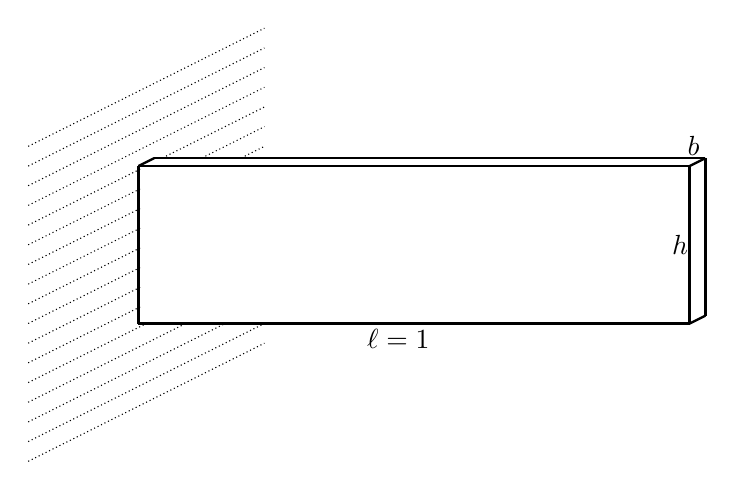
\begin{tikzpicture}
					\draw[line width = 0.3mm] (-0.1,1) -- (6.9,1);
					\draw[line width = 0.3mm] (-0.1,-1) -- (6.9,-1);
					\draw[line width = 0.3mm] (6.9,-1) -- (6.9,1);
					\draw[line width = 0.3mm] (-0.1,-1) -- (-0.1,1);
					
					\draw[line width = 0.3mm] (0.1,1.1) -- (7.1,1.1);
					\draw[line width = 0.3mm] (7.1,-0.9) -- (7.1,1.1);
					
					\draw[line width = 0.3mm] (-0.1,1) -- (0.1,1.1);
					\draw[line width = 0.3mm] (6.9,1) -- (7.1,1.1);
					\draw[line width = 0.3mm] (6.9,-1) -- (7.1,-0.9);
					
					
					
					\draw[scale=0.5, domain=-3:3, smooth, variable=\x,densely dotted] plot ({\x}, {0.5*\x+4});
					\draw[scale=0.5, domain=-3:3, smooth, variable=\x,densely dotted] plot ({\x}, {0.5*\x+3.5});
					\draw[scale=0.5, domain=-3:3, smooth, variable=\x,densely dotted] plot ({\x}, {0.5*\x+3});
					\draw[scale=0.5, domain=-3:3, smooth, variable=\x,densely dotted] plot ({\x}, {0.5*\x+2.5});
					
					\draw[scale=0.5, domain=-3:-0.1, smooth, variable=\x,densely dotted] plot ({\x}, {0.5*\x+2});
					\draw[scale=0.5, domain=-3:-0.1, smooth, variable=\x,densely dotted] plot ({\x}, {0.5*\x+1.5});
					\draw[scale=0.5, domain=-3:-0.1, smooth, variable=\x,densely dotted] plot ({\x}, {0.5*\x+1});
					
					\draw[scale=0.5, domain=0.5:3, smooth, variable=\x,densely dotted] plot ({\x}, {0.5*\x+2});
					\draw[scale=0.5, domain=1.5:3, smooth, variable=\x,densely dotted] plot ({\x}, {0.5*\x+1.5});
					\draw[scale=0.5, domain=2.5:3, smooth, variable=\x,densely dotted] plot ({\x}, {0.5*\x+1});
					
					\draw[scale=0.5, domain=-3:-0.1, smooth, variable=\x,densely dotted] plot ({\x}, {0.5*\x+0.5});
					\draw[scale=0.5, domain=-3:-0.1, smooth, variable=\x,densely dotted] plot ({\x}, {0.5*\x});
					\draw[scale=0.5, domain=-3:-0.1, smooth, variable=\x,densely dotted] plot ({\x}, {0.5*\x-0.5});
					\draw[scale=0.5, domain=-3:-0.1, smooth, variable=\x,densely dotted] plot ({\x}, {0.5*\x-1});
					\draw[scale=0.5, domain=-3:-0.1, smooth, variable=\x,densely dotted] plot ({\x}, {0.5*\x-1.5});
					\draw[scale=0.5, domain=-3:0, smooth, variable=\x,densely dotted] plot ({\x}, {0.5*\x-2});
					\draw[scale=0.5, domain=-3:1, smooth, variable=\x,densely dotted] plot ({\x}, {0.5*\x-2.5});
					\draw[scale=0.5, domain=-3:2, smooth, variable=\x,densely dotted] plot ({\x}, {0.5*\x-3});
					\draw[scale=0.5, domain=-3:3, smooth, variable=\x,densely dotted] plot ({\x}, {0.5*\x-3.5});
					\draw[scale=0.5, domain=-3:3, smooth, variable=\x,densely dotted] plot ({\x}, {0.5*\x-4});
					
					\node at (6.95,1.25) {$b$};
					\node at (6.78,0) {$h$};
					\node at (3.2,-1.2) {$\ell = 1$};
					

				\end{tikzpicture}
				\subcaption{Three-Dimensional Elastic Body}
				
			\end{minipage}
		}
	}
\end{figure}
\FloatBarrier

For both models the parameter $h$ represents the width of the beams. The three-dimensional model also have depth $b$. Intuitively, from the figure, the two-dimensional beam should compare better to the three-dimensional beam for smaller $b$.

\subsection{Accuracy of the numerical eigenvalues}
In the previous section, the accuracy of the two-dimensional beam's eigenvalues were investigated. This can be done similarly for the three-dimensional beam. The eigenvalues are also calculated using the Finite Element Method. Using piecewise tri-cubic basis functions, the following results were obtained.\\

For different values of $h$ and $b$, the first 30 eigenvalues are calculated with increasing grid sizes. The maximum relative error between the sets of eigenvalues are then calculated and graphed.\\

****************INSERT GRAPHIC**************\\

\subsection{Comparing the mode shapes}
In this section, the mode shapes of the two dimensional and three-dimensional beam are compared. Recall that beam-type eigenvalues are defined by \cite{LVV09} as any eigenvalue for which it's corresponding mode shape is similar to the mode shapes obtained in the Timoshenko beam theory.

\subsubsection{Mode shapes relating to beam type eigenvalues.}
Figure \ref{fig:beam-2dv3d} show some examples of beam type mode shapes for the displacement $u$.

\begin{figure}[h!]
	\scalebox{.8}{
		\makebox[\textwidth][c]{
			\centering
			\begin{minipage}[b]{0.8\linewidth}
				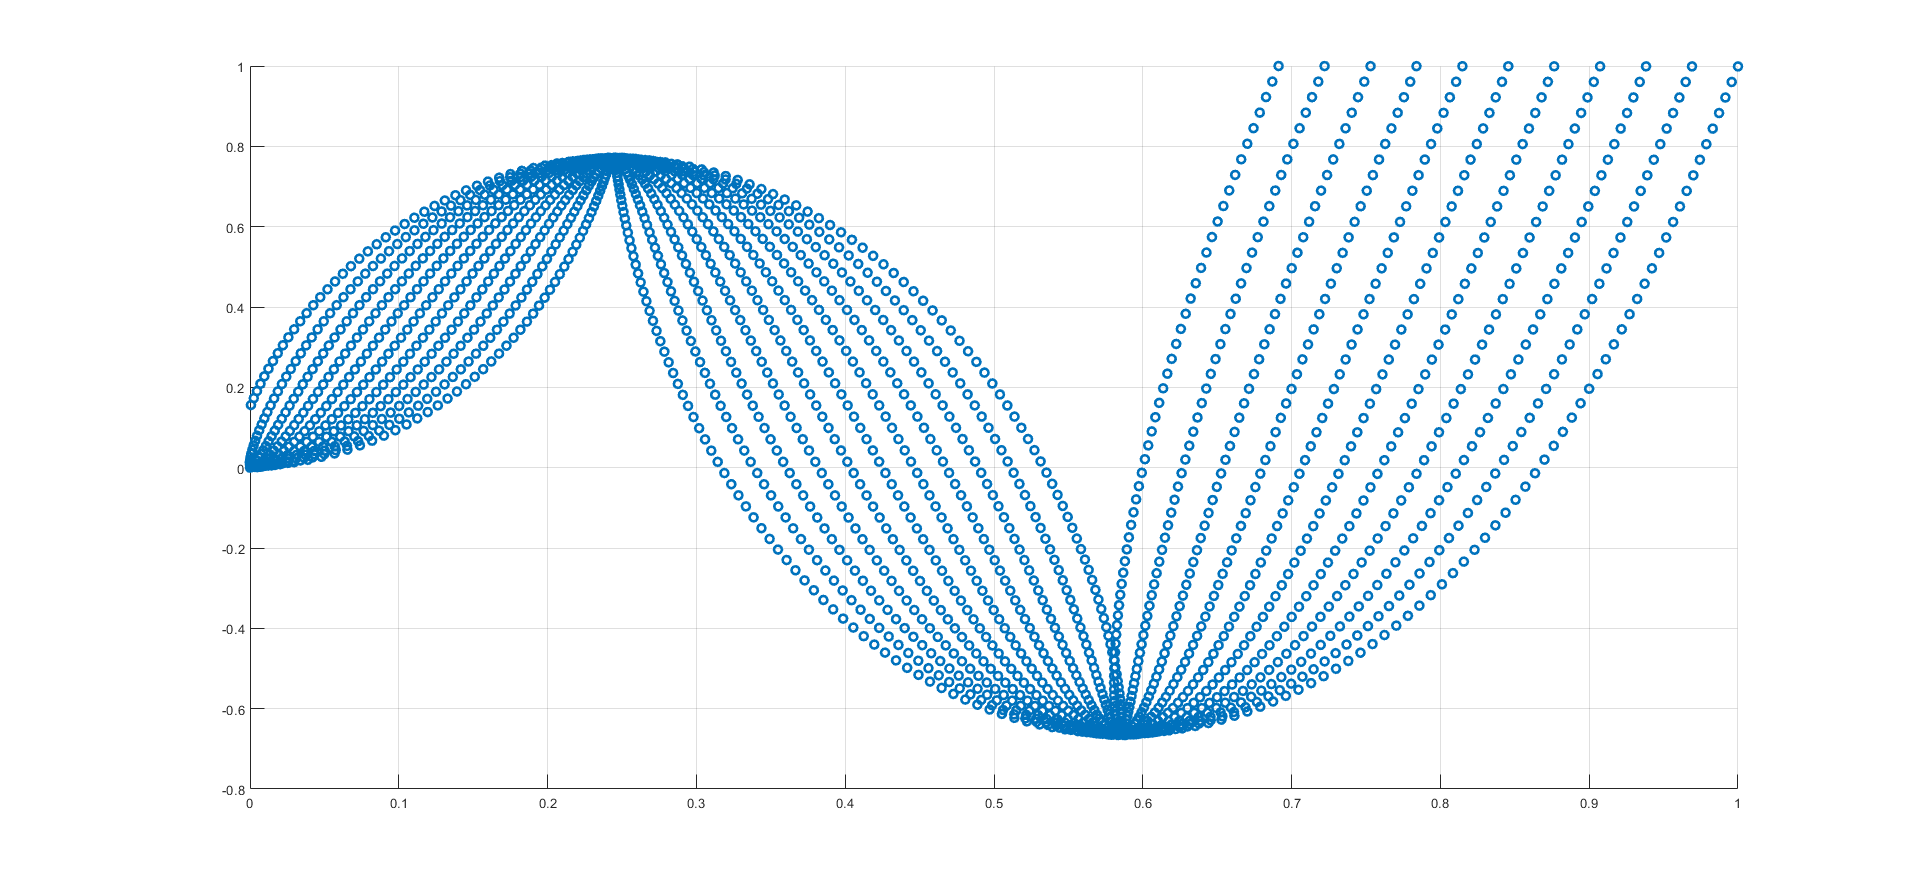
\includegraphics[width=1\linewidth]{3D12.png}
				\subcaption{3D Beam Type - $\lambda_{12} = 2.3293$}
				\label{fig:minipage2}
			\end{minipage}
			\begin{minipage}[b]{0.8\linewidth}
				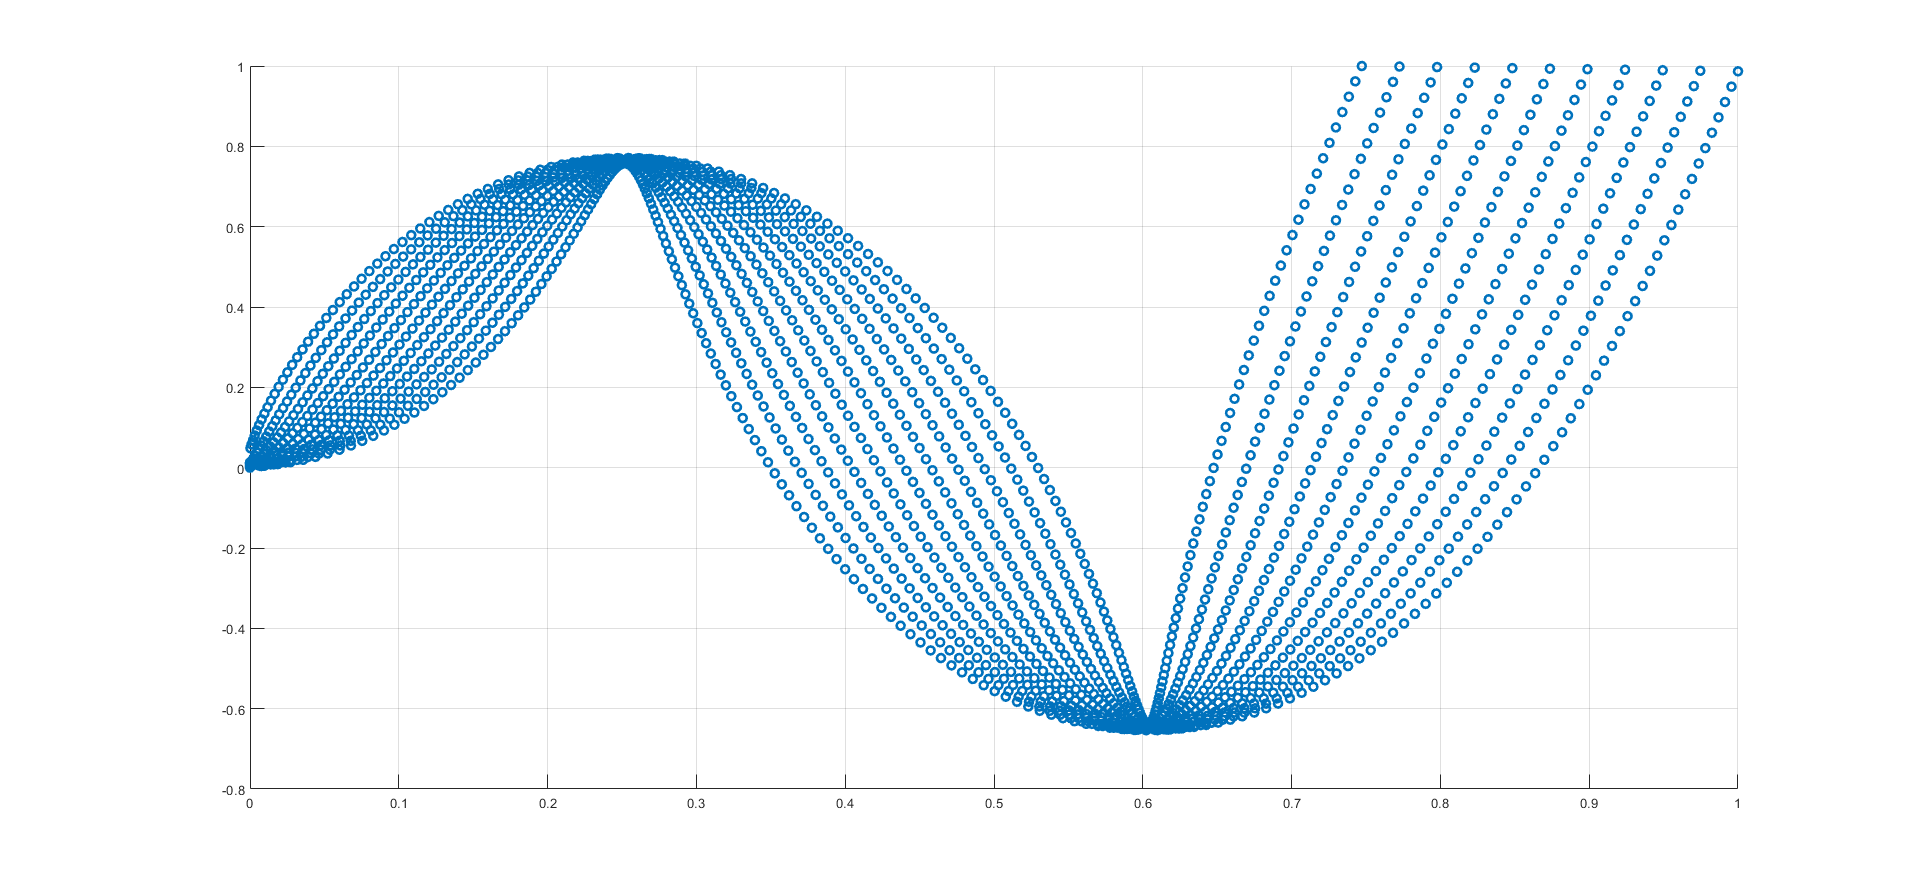
\includegraphics[width=1\linewidth]{2D3.png}
				\subcaption{2D Beam Type - $\lambda_3 = 2.3273$}
				\label{fig:minipage1}
			\end{minipage}
	}}
	\scalebox{.8}{
		\makebox[\textwidth][c]{
			\centering
			\begin{minipage}[b]{0.8\linewidth}
				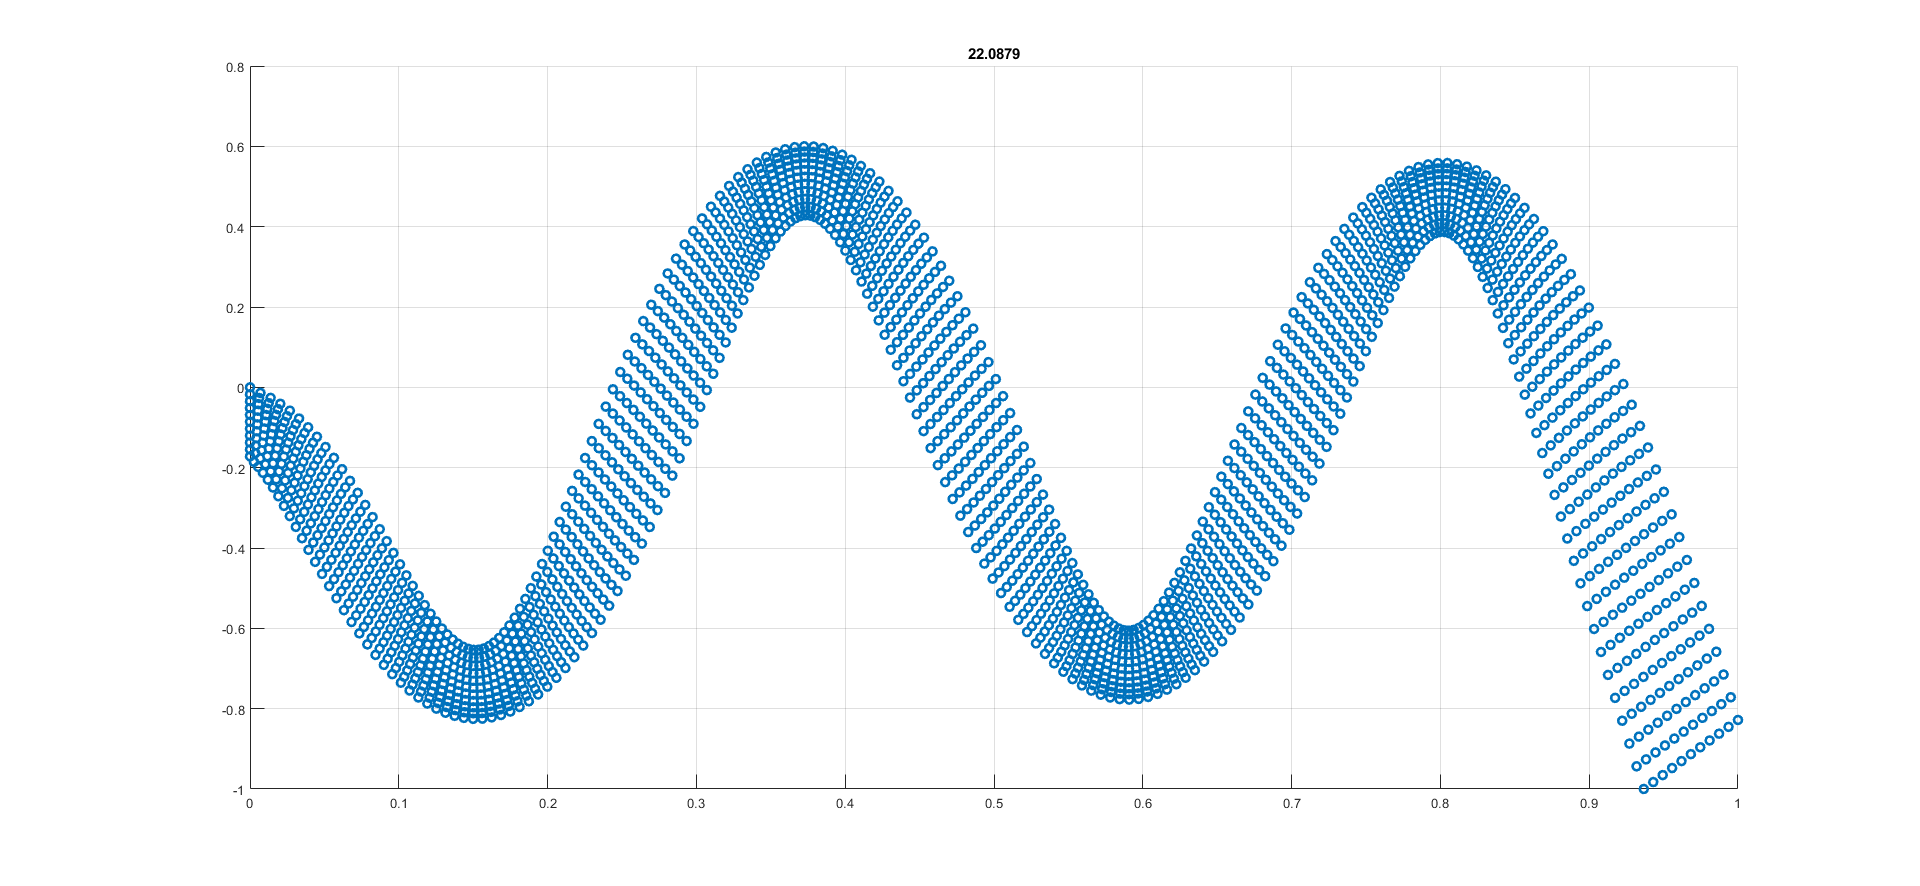
\includegraphics[width=1\linewidth]{3D22.png}
				\subcaption{3D Beam Type - $\lambda_{24} = 21.929$}
				\label{fig:minipage2}
			\end{minipage}
			\begin{minipage}[b]{0.8\linewidth}
				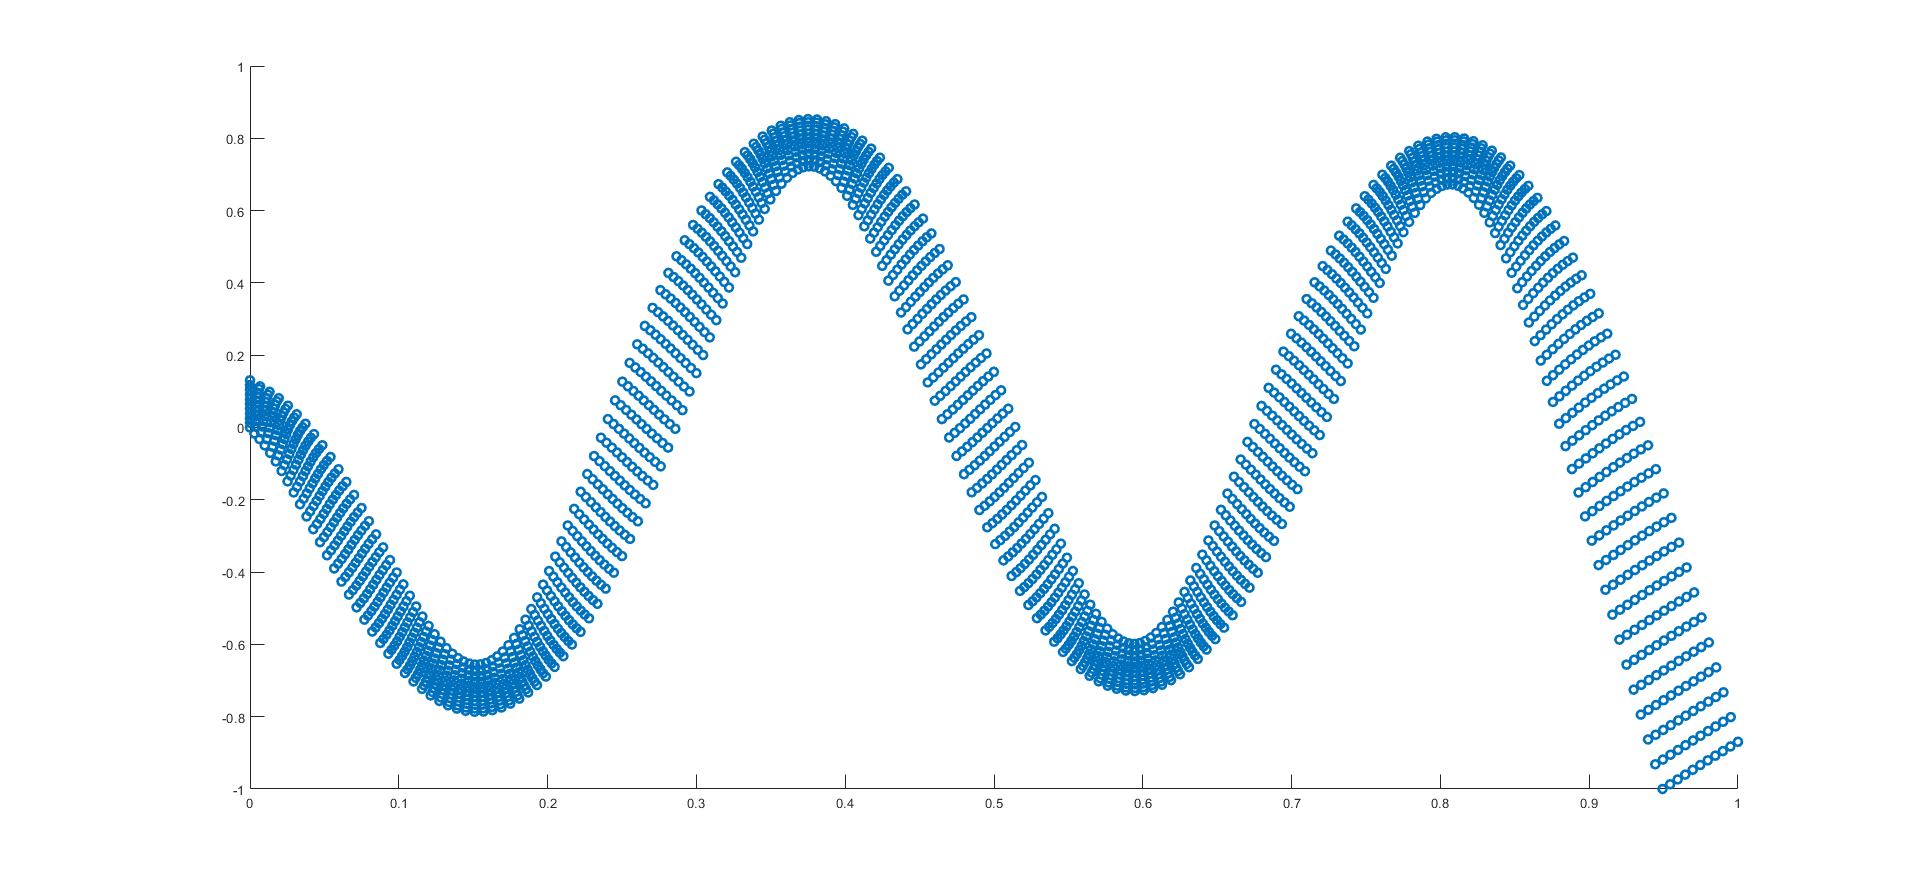
\includegraphics[width=1\linewidth]{2D6.png}
				\subcaption{2D Beam Type - $\lambda_6 = 21.911$}
				\label{fig:minipage1}
			\end{minipage}
			\caption{Mode shapes of the displacement $w$ with $h=1/20$.}
			\label{fig:beam-2dv3d}
	}}
\end{figure}
\FloatBarrier

\subsubsection{Mode shapes relating to non-beam type eigenvalues that are present in the two-dimensional model.}
Figure \ref{fig:nonbeam-2dv3d} show examples of mode shapes relating to non-beam type eigenvalues for the displacement $u$.

\FloatBarrier
\begin{figure}[h!]
	\scalebox{.8}{
		\makebox[\textwidth][c]{
			\centering
			\begin{minipage}[b]{0.8\linewidth}
				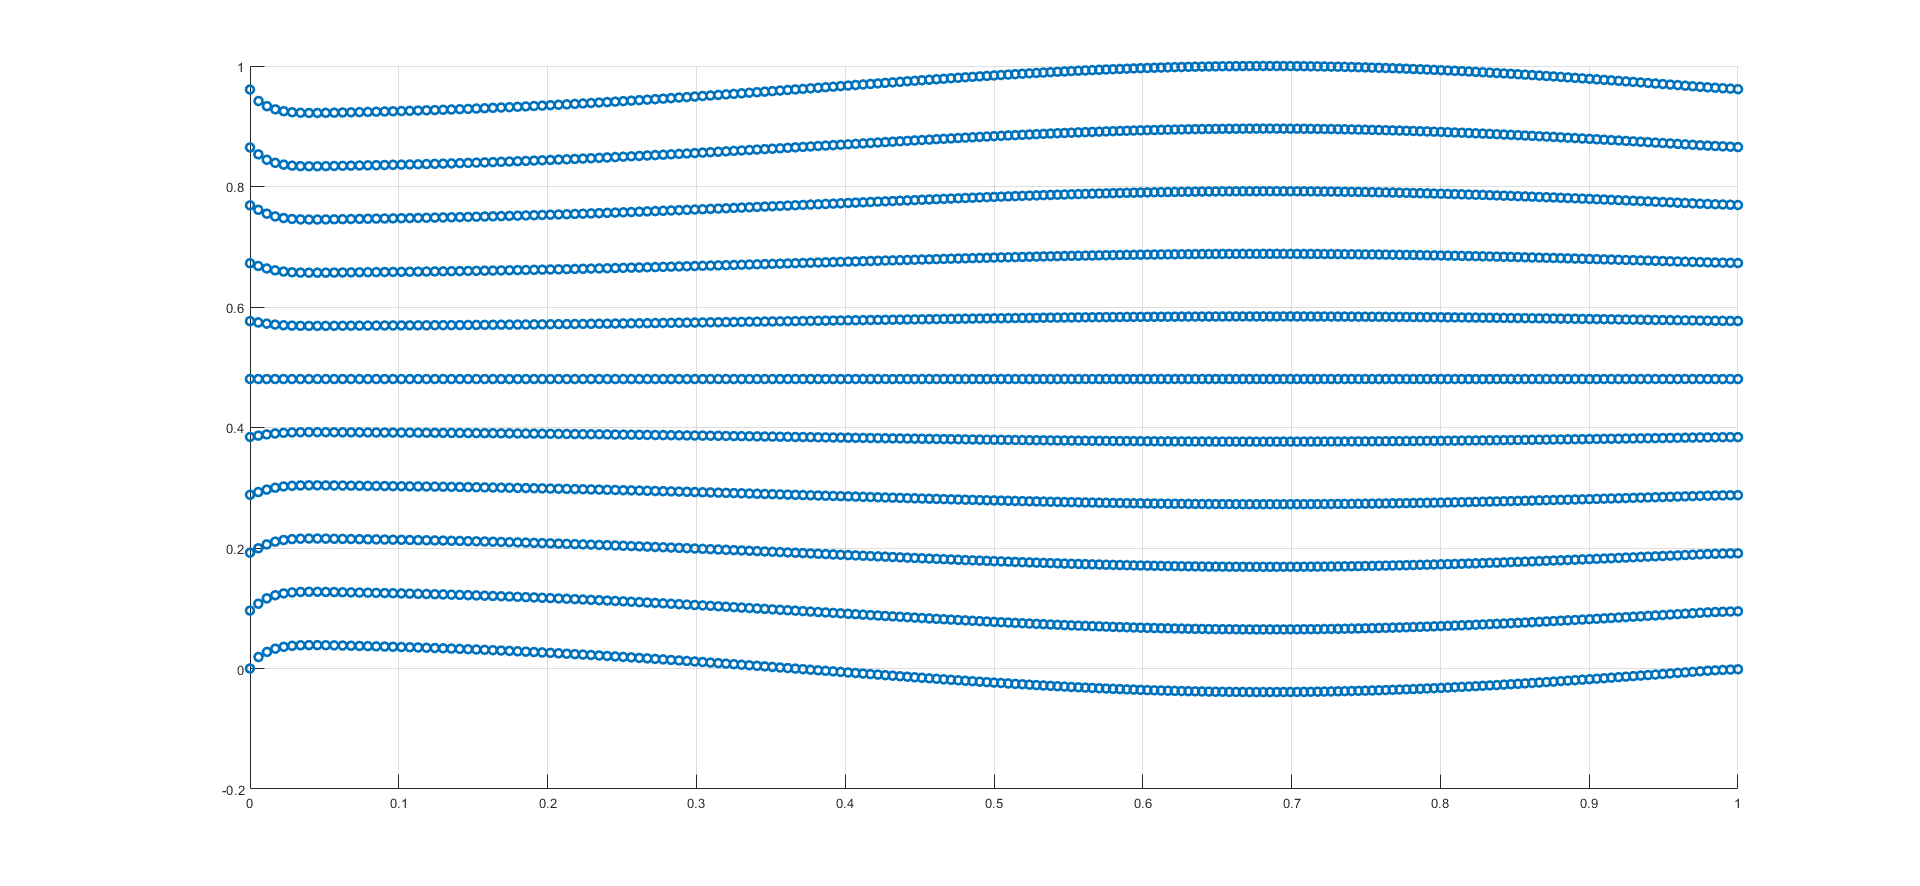
\includegraphics[width=1\linewidth]{3D33.png}
				\subcaption{3D Non-Beam Type - $\lambda_{33} = 69.374$}
				\label{fig:minipage2}
			\end{minipage}
			\begin{minipage}[b]{0.8\linewidth}
				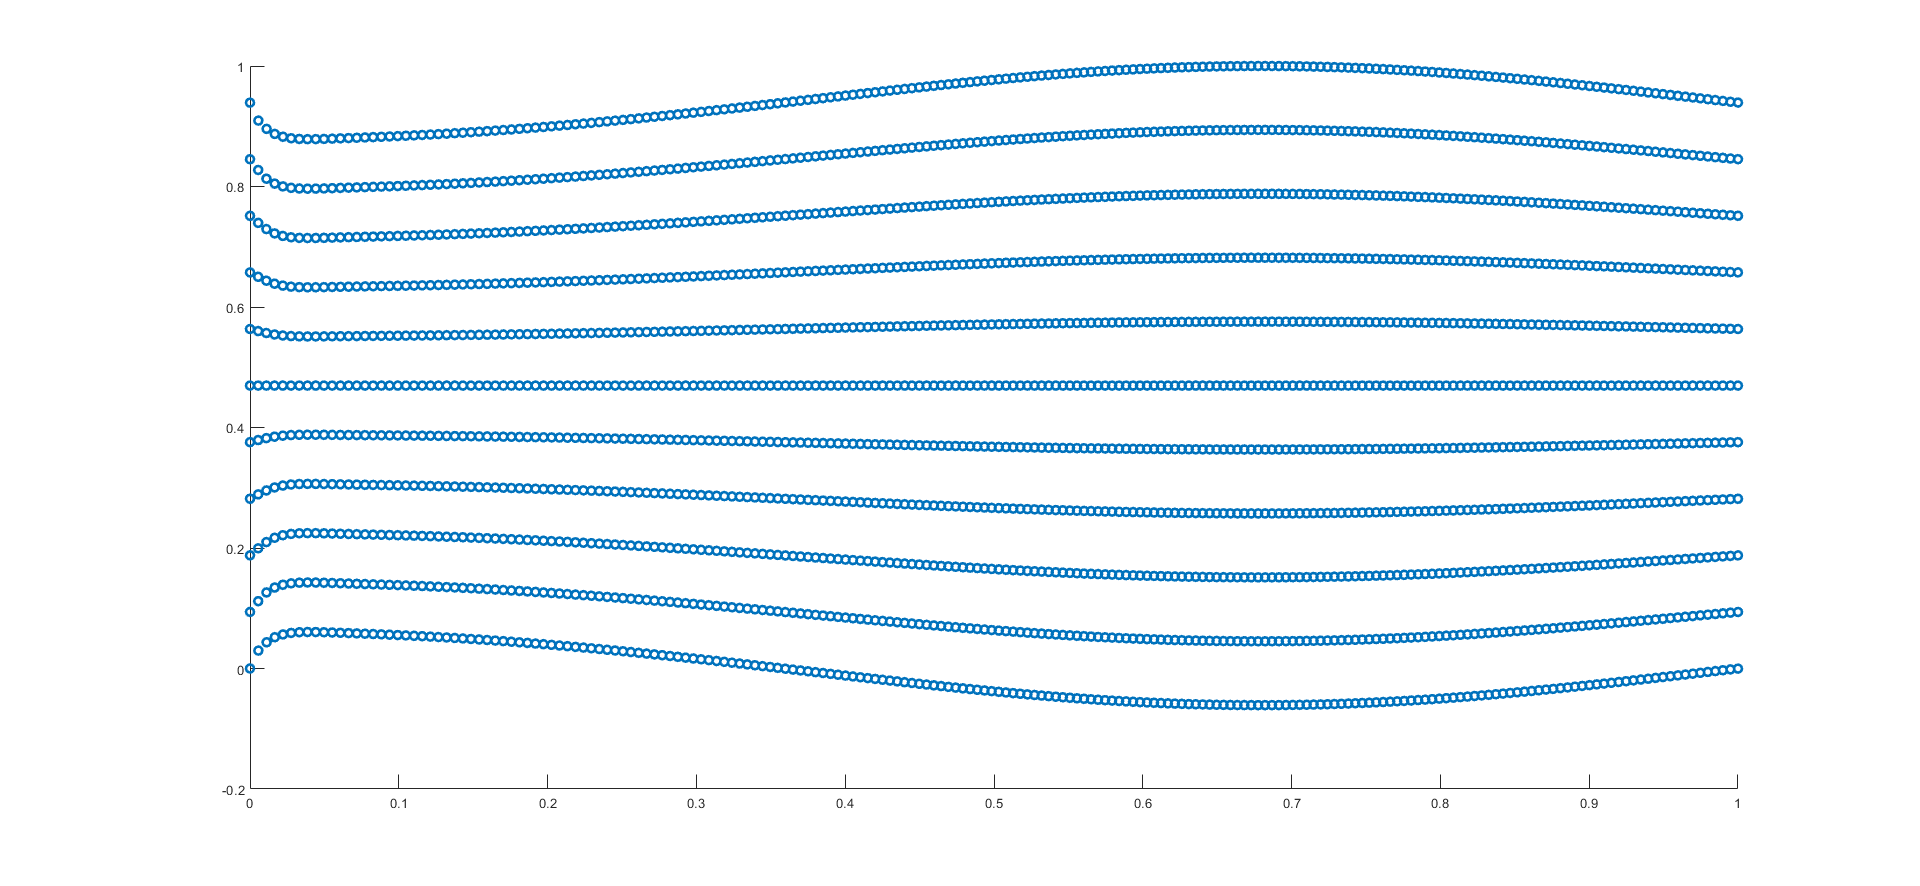
\includegraphics[width=1\linewidth]{2D8.png}
				\subcaption{2D Non-Beam Type - $\lambda_8 = 69.344$}
				\label{fig:minipage1}
			\end{minipage}
			\caption{Mode shapes of the displacement $w$ with $h=1/20$.}
			\label{fig:nonbeam-2dv3d}
	}}
\end{figure}
\FloatBarrier

\subsubsection{Mode shapes relating to non-beam type eigenvalues that are not present in the two-dimensional model.}
Figure \ref{fig:nonbeam-2dv3d} show examples of mode shapes relating to non-beam type eigenvalues for the displacement $u$ which are not present in the two-dimensional model. These mode shapes only appear in the three-dimensional beam.
\FloatBarrier
\begin{figure}[h!]
	\scalebox{.8}{
		\makebox[\textwidth][c]{
			\centering
			\begin{minipage}[b]{0.8\linewidth}
				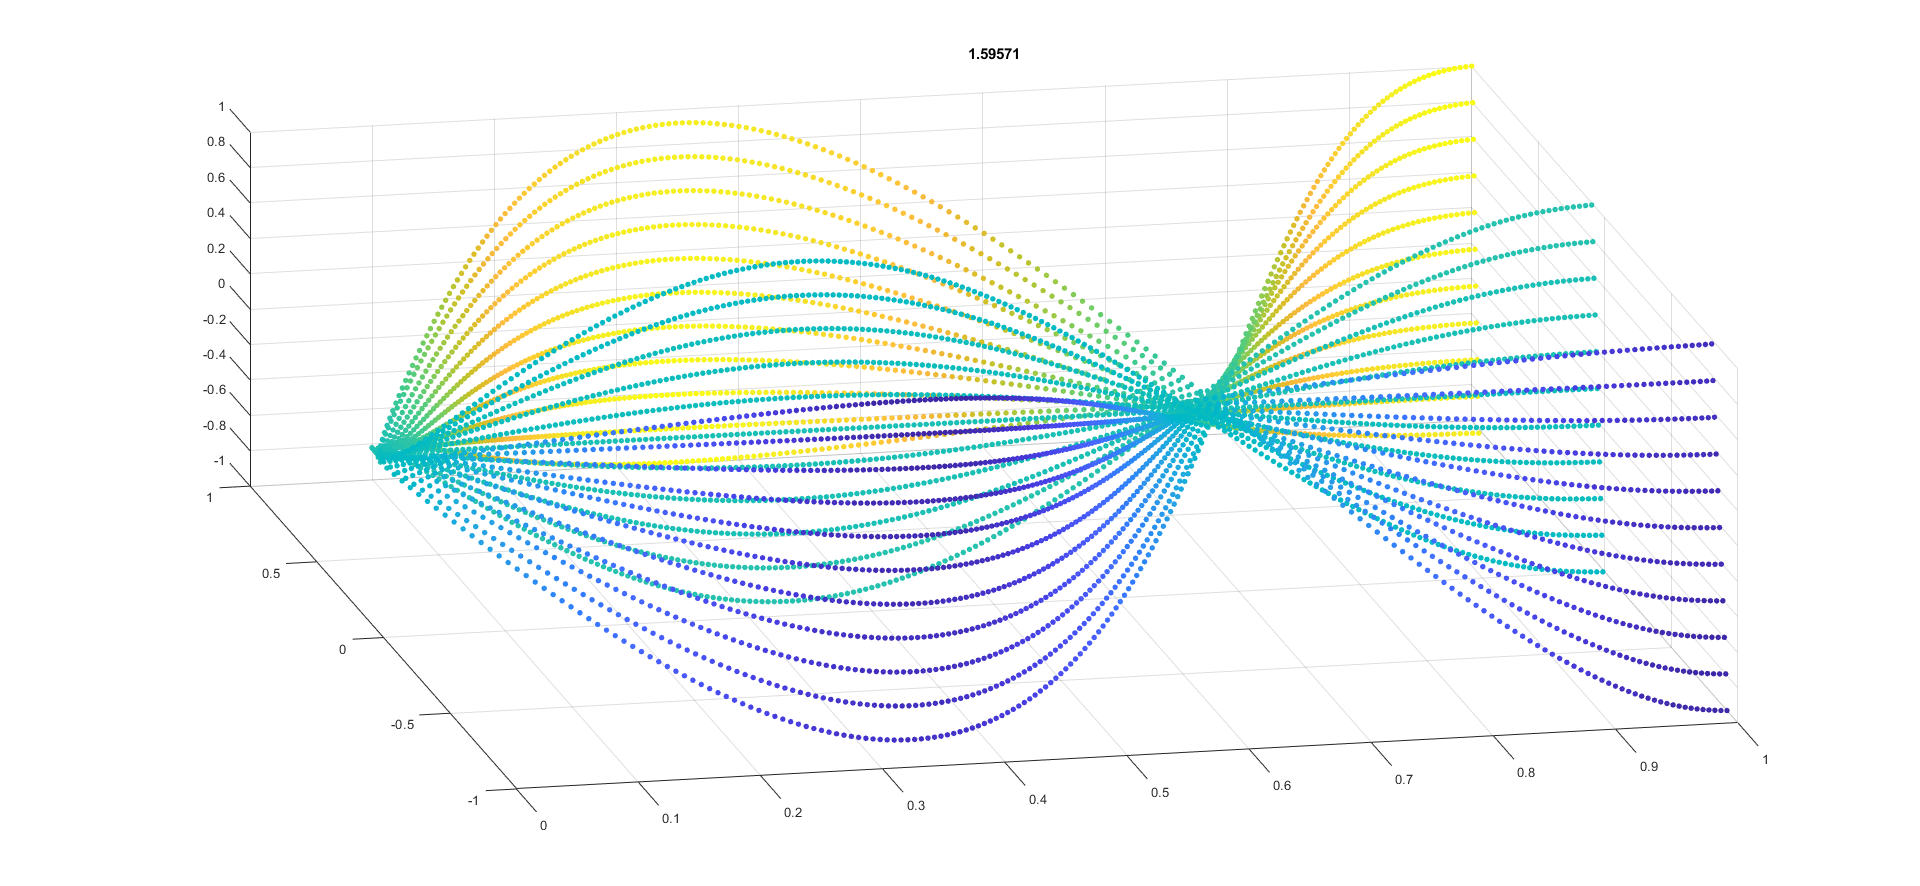
\includegraphics[width=1\linewidth]{3DNonBeam10.png}
				\subcaption{Non-2D Type - $\lambda_{10} = xx$}
				\label{fig:minipage2}
			\end{minipage}
			\begin{minipage}[b]{0.8\linewidth}
				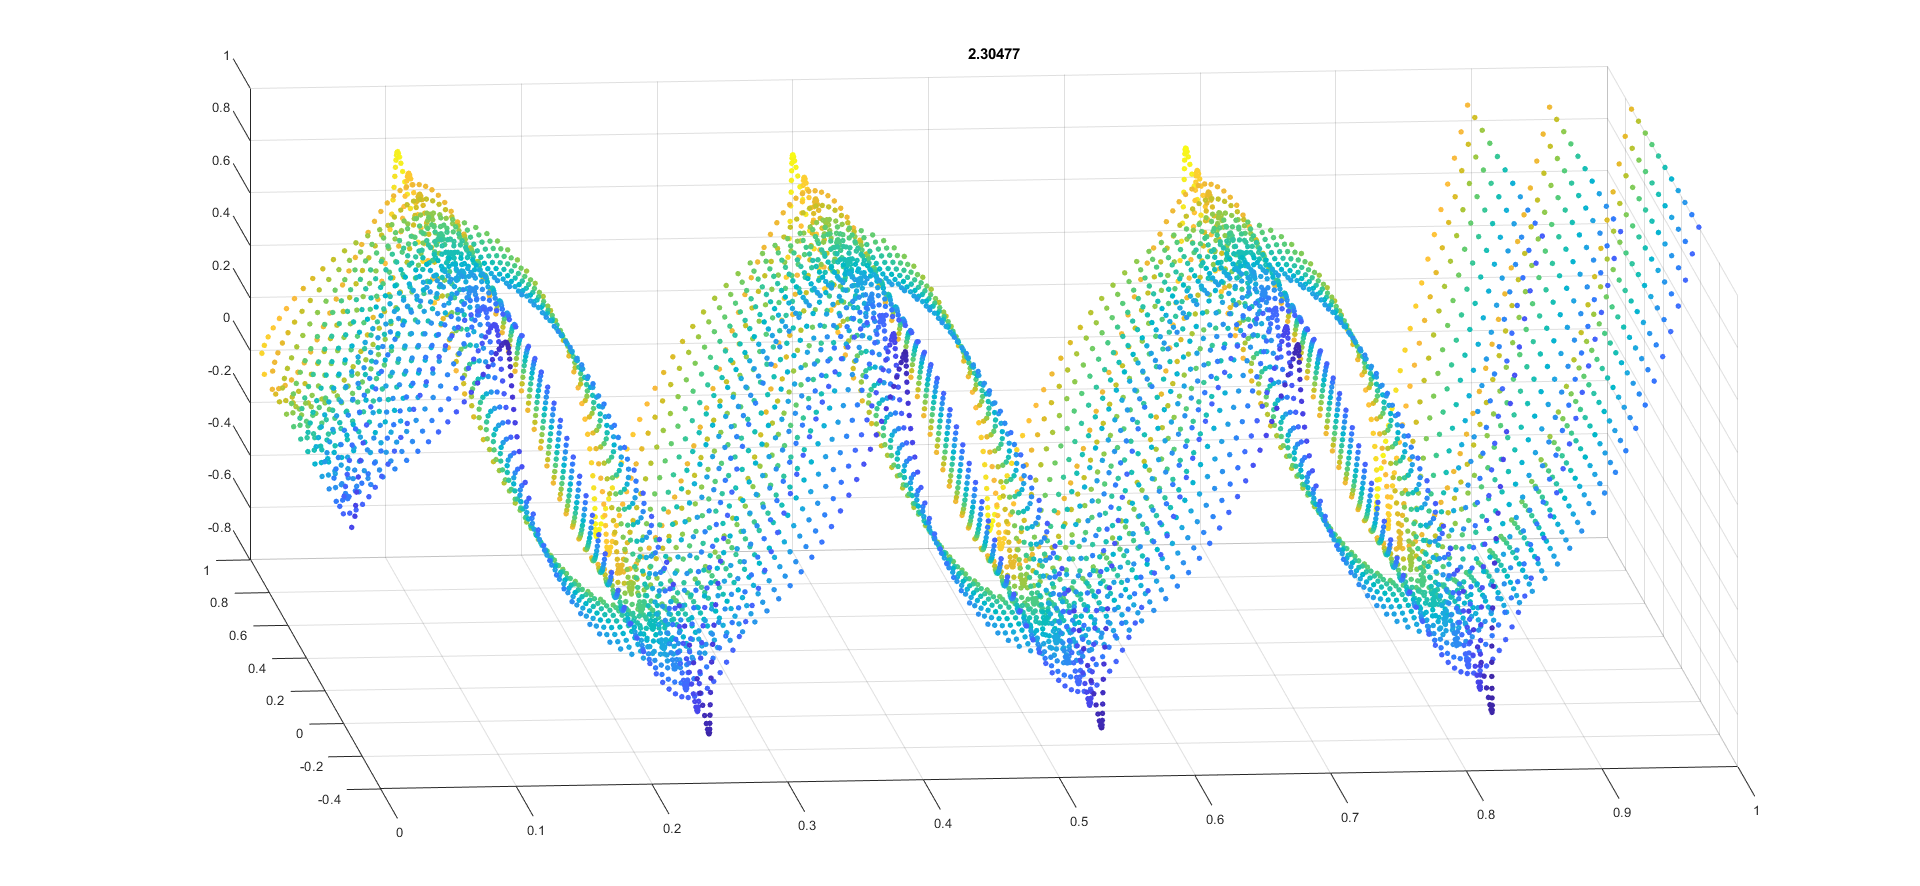
\includegraphics[width=1\linewidth]{3DNonBeam11.png}
				\subcaption{Non-2D Type - $\lambda_{11} = xx$}
				\label{fig:minipage11}
			\end{minipage}
			\caption{Mode shapes of the displacement $w$ with $\alpha = 4800$.}
			
	}}
\end{figure}
\FloatBarrier

Figure \ref{fig:minipage11} looks similar to the beam type eigenvalues, however the shape is in the $x-z$ axis.\\

\subsection{Comparing the eigenvalues}
The eigenvalues can now be compared. In the upcoming tables, the eigenvalues of the two-dimensional beam are compared to the eigenvalues of the three-dimensional beam. For each case of $h$, different values of $b$ are given.\\

Eigenvalues relating to non-beam type eigenvalues that are present in both the two-dimensional and three-dimensional beam, are highlighted in grey. The other non-beam type eigenvalues that are only found in the three-dimensional beam, are omitted from the tables. The original numbering is maintained.\\

The two cases for $h$ are $h = 1/5$ for a short beam and $1/20$ for a slender beam. For now, the investigation is restricted to values where $b \leq h$.

\begin{table}[htbp]
	\scalebox{.8}{
	\makebox[\textwidth]{
		\caption{Comparsion of Eigenvalues with $h = 1/5$.}
		\begin{tabular}{|cc|cc|cc|cc||cc|}
			\hline
			\multicolumn{10}{|c|}{Eigenvalues} \\
			\hline
			\hline
			i     & {b = h} & i     & {b = 1/2 h} & i     & {b = 1/4 h} & i     & {b = 1/8 h} & j     & 2D \\
			\hline
			{2} & 0.12307 & {2} & 0.12234 & {2} & 0.12198 & {3} & 0.12178 & 1     & 0.12151 \\
			{3} & 3.5773 & {5} & 3.5630 & {6} & 3.5558 & {8} & 3.5519 & 2     & 3.5460 \\
			\rowcolor{lightgray}{5} & 7.7799 & {6} & 7.7596 & {8} & 7.7471 & {11} & 7.7401 & 3     & 7.7311 \\
			{8} & 20.334 & {9} & 20.283 & {11} & 20.26 & {14} & 20.247 & 4     & 20.225 \\
			{10} & 56.247 & {12} & 56.173 & {15} & 56.156 & {22} & 56.142 & 5     & 56.109 \\
			\rowcolor{lightgray}{11} & 69.197 & {14} & 69.319 & {17} & 69.281 & {24} & 69.238 & 6     & 69.164 \\
			{14} & 114.03 & {16} & 114.01 & {20} & 114.05 & {29} & 114.06 & 7     & 114.03 \\
			\rowcolor{lightgray}{17} & 187.01 & {19} & 189.14 & {25} & 189.37 & {36} & 189.34 & 8     & 189.17 \\
			{18} & 192.21 & {20} & 192.41 & {26} & 192.58 & {37} & 192.63 & 9     & 192.61 \\
			{21} & 284.76 & {23} & 285.43 & {31} & 285.74 & {42} & 285.84 & 10    & 285.85 \\
			{23} & 327.57 & {26} & 328.24 & {35} & 328.37 & {46} & 328.40 & 11    & 328.40 \\
			\rowcolor{lightgray}{25} & 347.77 & {28} & 356.44 & {36} & 357.30 & {50} & 357.33 & 12    & 357.08 \\
			{27} & 393.69 & {30} & 396.84 & {38} & 397.28 & {53} & 397.37 & 13    & 397.33 \\
			{30} & 434.46 & {34} & 441.05 & {41} & 441.81 & {57} & 441.99 & 14    & 442.00 \\
			\rowcolor{lightgray}{31} & 523.65 & {36} & 534.04 & {43} & 534.17 & {63} & 534.03 & 15    & 533.71 \\
			{34} & 550.51 & {37} & 537.82 & {44} & 538.86 & {64} & 539.06 & 16    & 538.97 \\
			\rowcolor{lightgray}{37} & 590.86 & {41} & 587.43 & {48} & 594.17 & {65} & 595.58 & 17    & 596.06 \\
			{39} & 590.86 & {42} & 600.52 & {49} & 602.25 & {67} & 602.69 & 18    & 602.77 \\
			\rowcolor{lightgray}{42} & 646.21 & {44} & 657.22 & {50} & 658.04 & {71} & 658.06 & 19    & 657.87 \\
			{44} & 711.07 & {46} & 714.62 & {53} & 717.10 & {73} & 717.51 & 20    & 717.37 \\
			\hline
			\hline
			\multicolumn{2}{|c|}{Max RE: \  2.6069\%} &\multicolumn{2}{c|}{Max RE: \ 1.4469\%}  & \multicolumn{2}{c|}{Max RE: \  0.38192\%}  & \multicolumn{2}{c||}{Max RE: \ 0.22301\%}& \multicolumn{2}{c|}{-} \\
			\hline
		\end{tabular}%
		\label{tab:2v3_1}%
	}}
\end{table}%
\FloatBarrier
Table \ref{tab:2v3_1} show that the eigenvalues of the two-dimensional model compare very well to the three-dimensional model.  The maximum relative error decreases significantly as $b$ is decreased. Even with $b = h$ the maximum relative error is still less than $2.7\%$. \\

Table \ref{tab:2Dv3D_1_breakup} gives more information on the maximum relative error by separating the beam type and non-beam type eigenvalues.


% Table generated by Excel2LaTeX from sheet 'Sheet2'
\begin{table}[htbp]
	\centering
	\caption{****$h = 1/5$}
	\begin{tabular}{|c|cccc|}
		\hline
		\multicolumn{5}{|c|}{Maximum Relative Error} \\
		\hline
		\hline
		& {b = h} & {b = 1/2h} & {b = 1/4h} & {b = 1/8h} \\
		\hline
		Beam Type & 2.1420 \% & 0.6804 \% & 0.38192 \% & 0.22301 \% \\
		Non-Beam Type & 2.6069 \% & 1.4469 \% & 0.31546 \% & 0.11680 \% \\
		\hline
	\end{tabular}%
	\label{tab:2Dv3D_1_breakup}%
\end{table}%

From Table \ref{tab:2Dv3D_1_breakup}, it is clear that indeed for beam type eigenvalues, a short two-dimensional beam compares very well to a short three-dimensional beam.\\

\begin{table}[ht]
	\scalebox{.8}{
	\makebox[\textwidth]{
	\caption{Comparsion of Eigenvalues with $h = 1/20$. The non beam-type eigenvalues are highlighted or omitted.}
	\begin{tabular}{|cc|cc|cc|cc||cc|}
		\hline
		\multicolumn{10}{|c|}{Eigenvalues} \\
		\hline
		\hline
		i     & {b = h} & i     & {b = 1/2 h} & i     & {b = 1/4 h} & i     & {b = 1/8 h} & j     & 2D \\
		\hline
		{2} & 0.008043 & {2} & 0.008029 & {2} & 0.008023 & {3} & 0.00802 & {1} & {0.008013} \\
		{3} & 0.3087 & {4} & 0.30816 & {5} & 0.30794 & {7} & 0.30785 & {2} & {0.30757} \\
		{5} & 2.3357 & {8} & 2.3316 & {9} & 2.3300  & {12} & 2.3293 & {3} & {2.3273} \\
		\rowcolor{lightgray}{8} & 7.7217 & {10} & 7.7156 & {13} & 7.7124 & {16} & 7.7111 & {4} & {7.7077} \\
		{10} & 8.5387 & {11} & 8.5238 & {14} & 8.5182 & {18} & 8.516 & {5} & {8.5086} \\
		{11} & 21.986 & {14} & 21.948 & {18} & 21.934 & {24} & 21.929 & {6} & {21.911} \\
		{14} & 45.863 & {18} & 45.781 & {21} & 45.756 & {30} & 45.746 & {7} & {45.712} \\
		\rowcolor{lightgray}{17} & 69.444 & {19} & 69.408 & {25} & 69.385 & {33} & 69.374 & {8} & {69.344} \\
		{18} & 83.149 & {22} & 82.999 & {27} & 82.960 & {36} & 82.944 & {9} & {82.887} \\
		{21} & 136.44 & {25} & 136.19 & {31} & 136.14 & {42} & 136.12 & {10} & {136.03} \\
		\rowcolor{lightgray}{23} & 192.62 & {27} & 192.62 & {35} & 192.58 & {47} & 192.56 & {11} & {192.48} \\
		{25} & 207.87 & {29} & 207.5 & {36} & 207.43 & {48} & 207.41 & {12} & {207.29} \\
		{27} & 299.14 & {33} & 298.63 & {41} & 298.56 & {55} & 298.53 & {13} & {298.38} \\
		\rowcolor{lightgray}{30} & 376.68 & {35} & 377.01 & {44} & 377.01 & {58} & 376.98 & {14} & {376.83} \\
		{31} & 411.58 & {37} & 410.89 & {46} & 410.83 & {61} & 410.81 & {15} & {410.63} \\
		{34} & 546.15 & {40} & 545.27 & {50} & 545.24 & {66} & 545.23 & {16} & {545.03} \\
		\rowcolor{lightgray}{37} & 620.77 & {42} & 622.02 & {53} & 622.19 & {69} & 622.18 & {17} & {621.95} \\
		{39} & 703.55 & {44} & 702.49 & {54} & 702.29 & {71} & 702.53 & {18} & {702.31} \\
		{42} & 884.27 & {47} & 883.02 & {59} & 883.14 & {82} & 883.19 & {19} & {882.96} \\
		\rowcolor{lightgray}{44} & 923.68 & {49} & 926.88 & {60} & 927.43 & {86} & 927.50 & {20} & {927.18} \\
		\hline
		\hline
		\multicolumn{2}{|c|}{Max RE: \  0.37701\%} &\multicolumn{2}{c|}{Max RE: \ 0.19893\%}  & \multicolumn{2}{c|}{Max RE: \  0.12393\%}  & \multicolumn{2}{c||}{Max RE: \ 0.092843\%}& \multicolumn{2}{c|}{-} \\
		\hline
	\end{tabular}%
	\label{tab:2v3_2}%
}}
\end{table}%
\FloatBarrier

In Table \ref{tab:2v3_2}, the eigenvalues are again compared for $h = 1/20$. The maximum relative error shows very impressive results for this case. The maximum relative error is less than $0.4\%$ and the maximum relative error decreases as $b$ is decreased.\\

\begin{table}[htbp]
	\centering
	\caption{*****$h = 1/20$}
	\begin{tabular}{|c|cccc|}
		\hline
		\multicolumn{5}{|c|}{Maximum Relative Error} \\
		\hline
		\hline
		& {b = h} & {b = 1/2h} & {b = 1/4h} & {b = 1/8h} \\
		\hline
		Beam Type & 0.37701 \% & 0.19893 \% & 0.12393 \% & 0.092843 \% \\
		Non-Beam Type & 0.37682 \% & 0.10218 \% & 0.061213 \% & 0.043601 \% \\
		\hline
	\end{tabular}%
	\label{tab:2v3_2_split}%
\end{table}%
\FloatBarrier

Separating the errors of the beam-type eigenvalues and the non-beam type eigenvalues in Table \ref{tab:2v3_2_split}, just reaffirms the results.\\

Restricting the models where $b \leq h$ yielded great results. It has been shown that the two-dimensional beam compares very well the the three-dimensional beam. The comparison also improves for smaller values of $h$. This is a similar result as seen with the work of \cite{LVV09} in the previous section.

\subsection{$b > h$}
Now we can ask the question what happens if $b > h$. Of course for very large values of $b$, the question should be asked is if the beam model is still relevant. Therefore, the investigation will look at an incremental increase of $b$, without making assumptions on the relevancy of a beam model.\\

\FloatBarrier
\begin{table}[htbp]
	\scalebox{.8}{
	\makebox[\textwidth]{
		\caption{$h = 1/20$}
		\begin{tabular}{|cc|cc|cc||cc|}
			\hline
			\multicolumn{8}{|c|}{Eigenvalues} \\
			\hline
			\hline
			i     & {b = 2h} & i     & {b = 4h} & i     & {b = 8h} & j     & 2D \\
			\hline
			{2} & 0.008076 & {1} & 0.008162 & {1} & 0.008324 & 1     & 0.008013 \\
			{3} & 0.30995 & {3} & 0.31298 & {3} & 0.31738 & 2     & 0.30757 \\
			{5} & 2.3462 & {5} & 2.3737 & {6} & 2.4116 & 3     & 2.3273 \\
			\rowcolor{lightgray}{8} & 7.7312 & {8} & 7.7471 & {9} & 7.7711 & 4     & 7.7077 \\
			{10} & 8.5841 & {9} & 8.7082 & {10} & 8.7929 & 5     & 8.5086 \\
			{11} & 22.124 & {12} & 22.491 & {14} & 23.222 & 6     & 21.911 \\
			{14} & 46.195 & {14} & 47.003 & {18} & 47.921 & 7     & 45.712 \\
			\rowcolor{lightgray}{17} & 69.454 & {17} & 69.281 & {22} & 72.307 & 8     & 69.344 \\
			{18} & 83.822 & {18} & 85.218 & {24} & 80.607 & 9     & 82.887 \\
			{21} & 137.43 & {21} & 138.58 & {32} & 140.97 & 10    & 136.03 \\
			\hline
			\hline
			\multicolumn{2}{|c|}{Max RE: \  1.1289\%} &\multicolumn{2}{c|}{Max RE: \ 2.8261\%}  & \multicolumn{2}{c|}{Max RE: \  5.9821\%} & \multicolumn{2}{c|}{-} \\
			\hline
		\end{tabular}%
		\label{tab:b>h}%
	}}
\end{table}
\FloatBarrier
In Table \ref{tab:b>h}, $h = 1/20$ was chosen since it was the beam case investigated in the previous section and $b$ is increased by a factor of $2$. And here we see that the maximum relative error increases almost by a factor of $2$ for each case. Note also that this table only shows the first 10 eigenvalues.\\

There is also an increase of non-beam type eigenvalues that are only present in the three-dimensional model.\\

In Table \ref{tab:b>h-split}, the maximum relative error of the beam-type and non-beam type eigenvalues are separated.
\FloatBarrier
\begin{table}[htbp]
	\centering
	\caption{$\alpha = 4800$}
	\begin{tabular}{|c|ccc|}
		\hline
		\multicolumn{4}{|c|}{Maximum Relative Error} \\
		\hline
		\hline
		& {b = 2h} & {b = 4h} & {b = 8h} \\
		\hline
		Beam Type & 1.1289 \% & 2.8261 \% & 5.9821 \% \\
		Non-Beam Type & 0.30521 \% & 0.51096 \% & 4.2734 \% \\
		\hline
	\end{tabular}%
	\label{tab:b>h-split}%
\end{table}%
\FloatBarrier

From Table \ref{tab:b>h-split}, it is clear that as $b$ increases, the maximum relative error of the beam type eigenvalues increases and the two-dimensional model compares less to the three-dimensional model.\\

In this section, it has been shown that the two-dimensional beam compares very well to the three-dimensional beam, in practical beam problems. Practical beam problems imply that $b \leq h$. The models also compare much better if $h$ is smaller. For values of  $b > h$, the use of a beam model should be questioned.\\

For $b > h$, another model might be presented. In the next section, a Reisner-Mindlin plate model is investigated.
\end{document}



\begin{figure}[h!]\label{fig:compare:1D+2D}
	\scalebox{.8}{
		\makebox[\textwidth][c]{
			\caption{Side by side comparison of the beams.}
			\centering
			\begin{minipage}[b]{0.8\linewidth}
				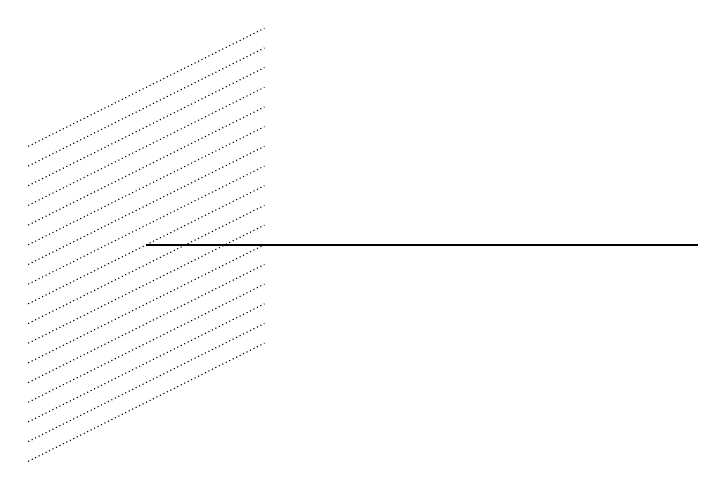
\begin{tikzpicture}
					\draw[line width = 0.3mm] (0,0) -- (7,0);
					
					\draw[scale=0.5, domain=-3:3, smooth, variable=\x,densely dotted] plot ({\x}, {0.5*\x+4});
					\draw[scale=0.5, domain=-3:3, smooth, variable=\x,densely dotted] plot ({\x}, {0.5*\x+3.5});
					\draw[scale=0.5, domain=-3:3, smooth, variable=\x,densely dotted] plot ({\x}, {0.5*\x+3});
					\draw[scale=0.5, domain=-3:3, smooth, variable=\x,densely dotted] plot ({\x}, {0.5*\x+2.5});
					\draw[scale=0.5, domain=-3:3, smooth, variable=\x,densely dotted] plot ({\x}, {0.5*\x+2});
					\draw[scale=0.5, domain=-3:3, smooth, variable=\x,densely dotted] plot ({\x}, {0.5*\x+1.5});
					\draw[scale=0.5, domain=-3:3, smooth, variable=\x,densely dotted] plot ({\x}, {0.5*\x+1});	
					\draw[scale=0.5, domain=-3:3, smooth, variable=\x,densely dotted] plot ({\x}, {0.5*\x+0.5});
					\draw[scale=0.5, domain=-3:3, smooth, variable=\x,densely dotted] plot ({\x}, {0.5*\x});
					\draw[scale=0.5, domain=-3:3, smooth, variable=\x,densely dotted] plot ({\x}, {0.5*\x-0.5});
					\draw[scale=0.5, domain=-3:3, smooth, variable=\x,densely dotted] plot ({\x}, {0.5*\x-1});
					\draw[scale=0.5, domain=-3:3, smooth, variable=\x,densely dotted] plot ({\x}, {0.5*\x-1.5});
					\draw[scale=0.5, domain=-3:3, smooth, variable=\x,densely dotted] plot ({\x}, {0.5*\x-2});
					\draw[scale=0.5, domain=-3:3, smooth, variable=\x,densely dotted] plot ({\x}, {0.5*\x-2.5});
					\draw[scale=0.5, domain=-3:3, smooth, variable=\x,densely dotted] plot ({\x}, {0.5*\x-3});
					\draw[scale=0.5, domain=-3:3, smooth, variable=\x,densely dotted] plot ({\x}, {0.5*\x-3.5});
					\draw[scale=0.5, domain=-3:3, smooth, variable=\x,densely dotted] plot ({\x}, {0.5*\x-4});
					
					%\node at (3.2,-0.2) {$\ell = 1$};
				\end{tikzpicture}
				\subcaption{Timoshenko Cantilever Beam}
			\end{minipage}
			\begin{minipage}[b]{0.8\linewidth}
				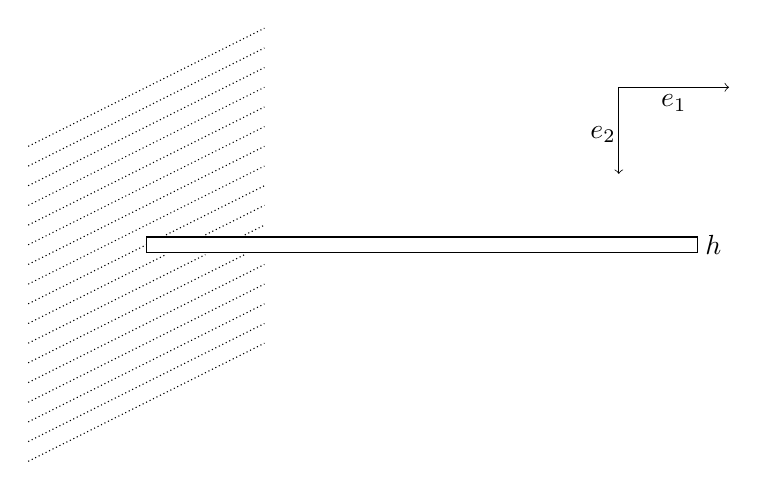
\begin{tikzpicture}
					\draw[line width = 0.2mm] (0,0.1) -- (7,0.1);
					\draw[line width = 0.2mm] (0,-0.1) -- (7,-0.1);
					\draw[line width = 0.2mm] (7,-0.1) -- (7,0.1);
					\draw[line width = 0.2mm] (0,-0.1) -- (0,0.1);
					
					\draw[scale=0.5, domain=-3:3, smooth, variable=\x,densely dotted] plot ({\x}, {0.5*\x+4});
					\draw[scale=0.5, domain=-3:3, smooth, variable=\x,densely dotted] plot ({\x}, {0.5*\x+3.5});
					\draw[scale=0.5, domain=-3:3, smooth, variable=\x,densely dotted] plot ({\x}, {0.5*\x+3});
					\draw[scale=0.5, domain=-3:3, smooth, variable=\x,densely dotted] plot ({\x}, {0.5*\x+2.5});
					\draw[scale=0.5, domain=-3:3, smooth, variable=\x,densely dotted] plot ({\x}, {0.5*\x+2});
					\draw[scale=0.5, domain=-3:3, smooth, variable=\x,densely dotted] plot ({\x}, {0.5*\x+1.5});
					\draw[scale=0.5, domain=-3:3, smooth, variable=\x,densely dotted] plot ({\x}, {0.5*\x+1});
					\draw[scale=0.5, domain=-3:3, smooth, variable=\x,densely dotted] plot ({\x}, {0.5*\x+0.5});
					
					\draw[scale=0.5, domain=-3:0, smooth, variable=\x,densely dotted] plot ({\x}, {0.5*\x});
					\draw[scale=0.5, domain=-3:0.5, smooth, variable=\x,densely dotted] plot ({\x}, {0.5*\x-0.5});
					\draw[scale=0.5, domain=-3:1.5, smooth, variable=\x,densely dotted] plot ({\x}, {0.5*\x-1});
					\draw[scale=0.5, domain=-3:2.5, smooth, variable=\x,densely dotted] plot ({\x}, {0.5*\x-1.5});
					
					\draw[scale=0.5, domain=0.5:3, smooth, variable=\x,densely dotted] plot ({\x}, {0.5*\x});
					\draw[scale=0.5, domain=1.5:3, smooth, variable=\x,densely dotted] plot ({\x}, {0.5*\x-0.5});
					\draw[scale=0.5, domain=2.5:3, smooth, variable=\x,densely dotted] plot ({\x}, {0.5*\x-1});
					
					
					\draw[scale=0.5, domain=-3:3, smooth, variable=\x,densely dotted] plot ({\x}, {0.5*\x-2});
					\draw[scale=0.5, domain=-3:3, smooth, variable=\x,densely dotted] plot ({\x}, {0.5*\x-2.5});
					\draw[scale=0.5, domain=-3:3, smooth, variable=\x,densely dotted] plot ({\x}, {0.5*\x-3});
					\draw[scale=0.5, domain=-3:3, smooth, variable=\x,densely dotted] plot ({\x}, {0.5*\x-3.5});
					\draw[scale=0.5, domain=-3:3, smooth, variable=\x,densely dotted] plot ({\x}, {0.5*\x-4});
					
					\draw[line width = 0.1mm,->] (6,2) -- (7.4,2);
					\draw[line width = 0.1mm,->] (6,2) -- (6,0.9);
					\node at (6.7,1.8) {$e_1$};
					\node at (5.8,1.4) {$e_2$};
					
					\node at (7.2,0) {$h$};
					%\node at (3.2,-0.3) {$\ell = 1$};
					
				\end{tikzpicture}
				\subcaption{Two-Dimensional Cantilever Beam}
			\end{minipage}
		}
	}
\end{figure}
